В данной главе рассматривается задача выбора структуры модели глубокого обучения. Предлагается ввести вероятностные предположения о распределении параметров и распределении структуры модели. 
Проводится градиентная оптимизация параметров и гиперпараметров модели на основе байесовского вариационного вывода.  В качестве оптимизируемой функции для гиперпараметров модели предлагается обобщенная функция ее обоснованности. Показано, что данная функция оптимизирует ряд критериев выбора структуры модели: метод максимального правдоподобия, последовательное увеличение и снижению сложности модели, полный перебор структуры модели, а также получение максимума вариационной оценки обоснованности модели. Решается двухуровневая задача оптимизации: на первом уровне проводится оптимизация нижней оценки обоснованности модели по вариационным параметрам модели. На втором уровне проводится оптимизация гиперпараметров модели.

\section{Вероятностная модель}
Определим априорные распределения параметров и структуры модели следующим образом.
Пусть для каждого ребра $(j,k) \in E$ и каждой базовой функции $\mathbf{g}^{j,k}_l$ параметры модели $\w^{j,k}_l$ распределены нормально с нулевым средним:
\[
    \w^{j,k}_l \sim \mathcal{N}\bigl(\mathbf{0}, (\gamma^{j,k}_l)^2(\A^{j,k}_l)^{-1}\bigr),
\]
где $ (\A^{j,k}_l)^{-1}$ --- диагональная матрица, $l \in \{1,\dots,K^{j,k}\}$, где $K^{j,k}$ --- количество базовых функций для ребра $K^{j,k}$. Априорное распределение $p(\w|\G, \h)$ параметров $\w^{j,k}_l$ зависит не только от гиперпараметров $\A_k^{j,k}$, но и от структурного параметра $\gamma^{j,k}_l \in (0,1)$.


В качестве априорного распределения для структуры $\G$ предлагается использовать произведение распределений Gumbel-Softmax ($\mathcal{GS}$)~\cite{gumbel}:
\[
    \priorG = \prod_{(j,k) \in E} p(\g^{j,k}|\s^{j,k}, \lamT), \quad 
\]
где для каждого структурного параметра $\g^{j,k}$ с количеством базовых функций $K^{j,k}$ вероятность $p(\g^{j,k}|\s^{j,k}, \lamT)$ определена следующим образом:
\begin{multline}
\label{eq:gs_pdf}
    p(\g^{j,k}|\s^{j,k}, \lamT) = (K^{j,k}-1)!(\lamT)^{K^{h,j}-1}\prod_{l=1}^{K^{j,k}} s^{j,k}_l(\g^{j,k}_l)^{-\lamT -1} \times \\ \times \left(\sum_{l=1}^{K^{j,k}} s^{j,k}_l(\g^{j,k}_l)^{-\lamT}\right)^{-K^{j,k}},
\end{multline}
где $\s^{j,k} \in (0,\infty)^K{^{j,k}}$ --- гиперпараметр, отвечающий за смещенность плотности распределения относительно точек симплекса на $K^{j,k}$ вершинах, $\lamT > 0$ --- метапараметр температуры, отвечающий за концентрацию плотности вблизи вершин симплекса или в центре симплекса.

Перечислим свойства, которыми обладает распределение Gumbel-Softmax:
\begin{enumerate}
\item  Компонента  $l$ случайной величины $\g^{j,k}$ представима следующим образом:
\begin{equation}
\label{eq:gs_sample}
    {\g}^{j,k}_l = \frac{\text{exp}(\log s^{j,k}_l+{G}^{j,k}_l)/\lamT}{\sum_{l'=1}^{K^{j,k}}\text{exp}(\log s^{j,k}_{l'}+{G}^{j,k}_{l'})/\lamT},
\end{equation}
где $\mathbf{G}^{j,k} \sim -\log \bigl(-\log\mathcal{U}(0,1)^{K^{j,k}}\bigr).$ 

\item Свойство округления: $p(\g_{l_1} > \g_{l_2}, l_1\neq l_2|\s^{j,k}, \lamT) = \frac{s^{j,k}_{l_1}}{\sum_{l'}s^{j,k}_{l'}}.$

\item При устремлении температуры к нулю  плотность случайной величины концентрируется на вершинах симплекса:
\[
p(\lim_{\lamT \to 0} {\gamma}^{j,k}_{l}= 1|\s^{j,k}, \lamT)=\frac{s^{j,k}_l}{\sum_{l'}s^{j,k}_{l'}}.
\]


\item При устремлении температуры к бесконечности плотность распределения концентрируется в центре симплекса:
\begin{equation}
\label{eq:theorem_gs}
    \lim_{\lamT \to \infty}  p(\g^{j,k}|\s^{j,k}, \lamT) = 
    \begin{cases}
    \infty, \g^{j,k} = \frac{1}{K^{j,k}}, l \in \{1,\dots,K^{j,k}\},\\
    0, \text{ иначе.}
    \end{cases}
\end{equation}
\end{enumerate}

Доказательства первых трех утверждений приведены в~\cite{gumbel}. Докажем утверждение 4.

\begin{proof} 
Формула плотности с точностью до множителя записывается следующим образом :
\begin{equation}
\label{eq:pdf_proof}
    p(\g^{j,k}|\s^{j,k}, \lamT) \propto    \frac{(\lamT)^{K^{j,k}-1}}{\left(\sum_{l=1}^{K^{j,k}} s^{j,k}_l(\g^{j,k}_l)^{-\frac{K^{j,k}-1}{K^{j,k}}\lamT}\prod_{l'=1}^{K^{j,k}} [l \neq l'](\g_l^{j,k})^{\frac{1}{K^{j,k}}\lamT}\right)^{K^{j,k}}}.
\end{equation}

Заметим, что числитель $(\lamT)^{K^{j,k}-1}$ имеет меньшую скорость сходимости, чем знаменатель, поэтому для вычисления предела достаточно проанализировать только знаменатель. Знаменатель под степенью $(K^{j,k})$ представляется суммой слагаемых следующего вида: 
\begin{equation}
\label{eq:gs}
    \left(\frac{\prod_{l' \neq l} \gamma_{l'}^{\frac{1}{K^{j,k}}}}{\gamma_l^{\frac{K^{j,k}-1}{K^{j,k}}}}\right)^{\lamT}.
\end{equation}

Рассмотрим два случая: когда вектор $\g^{j,k}$  лежит не в центре симплекса, и когда  $\g^{j,k}$ лежит в центре симплекса. 
Пусть хотя бы для одной компоненты $l$ выполнено: $\g^{j,k}_l \neq \frac{1}{K^{j,k}}$. Пусть $l'$ соответствует индексу максимальной компоненты вектора $\g^{j,k}$:
\[
    \l' = \argmax_{l \in \{1,\dots,K^{j,k}\}} \g^{j,k}_l.
\]
Для $l=l'$ предел выражения~\eqref{eq:gs} при $\lamT \to \infty$ стремится к бесконечности. Для $l\neq l'$ предел выражения~\eqref{eq:gs} при $\lamT \to \infty$ стремится к нулю. Возводя сумму пределов в степень $(-K^{j,k})$ получаем предел плотности, равный нулю.

Рассмотрим второй случай. Пусть ${\gamma}^{j,k}_l = \frac{1}{K^{j,k}}$ для всех компонент вектора $\g^{j,k}$.
Тогда выражение~\eqref{eq:gs_pdf} с точностью до множителя упрощается до $(\lamT)^{K^{j,k}-1}$. Предел данного выражения стремится к бесконечности.
Таким образом, предел плотности Gumbel-Softmax равен выражению~\eqref{eq:theorem_gs}, что и требовалось доказать.

\end{proof}


Первое свойство Gumbel-Softmax распределения позволяет использовать репараметризацию при вычислении градиента в вариационном выводе (англ. reparametrization trick). 
\begin{defin} Случайную величину  $\psi$ с распределением $q$ с параметрами $\teta_\psi$ назовем репараметризованной через случайную величину $\varepsilon$, чье распределение не зависит от параметров $\teta_\psi$, если:
\[
   \psi = g(\varepsilon, \teta_\psi)
\]
где  $g$ --- некоторая непрерывная функция.
\end{defin}

Идею репараметризации поясним на следующем примере.
\begin{example} Пусть структура $\G$ зафиксирована для модели $\model$. Рассмотрим математическое ожидание логарифма правдоподобия выборки модели по некоторому непрерывному распределению $\qw$:
\[
    \E_{\qw} \log~\LL=  \int_{\w} \log~\LL \qw d\w.
\]
Продифференцируем данное выражение по параметрам $\tetaw$ вариационного распределения $\qw$, полагая что оно удовлетворяет необходимым условиям для переноса оператора дифференцирования под знак интеграла:
\[
    \nabla_{\tetaw} \E_{\qw} \log \LL = 
\int_{\w}  \log \LL \nabla_{\tetaw}\qw d\w.
\]
Это выражение в общем виде не имеет аналитического решения. Пусть распределение $\qw$ для параметров $\mathbf{w}$ подлежит репараметризации через случайную величину $\boldsymbol{\varepsilon}$:
\[
    \w = \mathbf{g}(\boldsymbol{\varepsilon}, \tetaw).
\] 
Тогда справедливо следующее выражение:
\[
 \nabla_{\tetaw} \E_{\q} \log \LL = \nabla_{\tetaw} \E_{\boldsymbol{\varepsilon}} \log \LL [][][\mathbf{g}(\boldsymbol{\varepsilon})] =
\]
\[= \int_{\boldsymbol{\varepsilon}}\nabla_{\tetaw} \log\LL [][][\mathbf{g}(\boldsymbol{\varepsilon})] p(\boldsymbol{\varepsilon}) d\boldsymbol{\varepsilon}=\E_{\boldsymbol{\varepsilon}} \nabla_{\teta} \log\LL [][][\mathbf{g}(\boldsymbol{\varepsilon})].\]
Таким образом, распределение, позволяющее произвести репараметризацию, является более удобным для вычисления интегральных оценок вида $ \nabla_{\tetaw} \E_{\q} \log \LL$, а также позволяет повысить точность приближенного вычисления значений таких функций~\cite{reparametrization}.
Подробный анализ репараметризации для генеративных моделей глубокого обучения представлен в~\cite{reparametrization_blog}.
% отсюда: http://gregorygundersen.com/blog/2018/04/29/reparameterization/
\end{example}

Пример распределения Gumbel-Softmax при различных параметрах представлен на Рис.~\ref{fig:gs}. В качестве альтернативы для априорного распределения структуры выступает  распределение Дирихле. В качестве предельного случая, когда все структуры $\G \in \Gb$ равнозначны, выступает равномерное распределение. Выбор в качестве распределения стрктуры произведения распределений Gumbel-Softmax  обоснован выбором этого распределения в качестве вариационного. 

\begin{figure}
 \begin{minipage}[t]{.2\textwidth}
        \centering
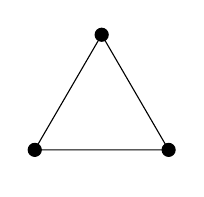
\begin{tikzpicture}[%
x={(1.7cm,0cm)},
y={(0cm,1.7cm)},
]

\coordinate (A) at (0,0); 
\coordinate (B) at (1,0) ;
\coordinate (C) at (0.5,0.86); 

%Ecken
\node[circle,scale=0.5,fill=black,draw=black](Ap) at (0,0){};
\node[circle,scale=0.5,fill=black,draw=black](Bp) at (1,0){};
\node[circle,scale=0.5,fill=black,draw=black](Cp) at (0.5,0.86){};

%Kanten
\draw[] (A)
-- (B)  node[midway, below]{}
-- (C)      node[midway, right]{}
-- (A)  node[midway, left]{};

\end{tikzpicture}
\subcaption{}
\end{minipage}
\hfill
 \begin{minipage}[t]{.2\textwidth}
   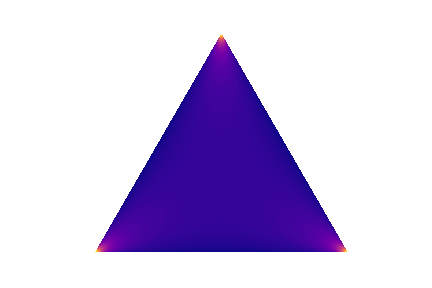
\includegraphics[width=\textwidth]{plots/notebooks/gs1.png}
\subcaption{}
\end{minipage}
\hfill
 \begin{minipage}[t]{.2\textwidth}
   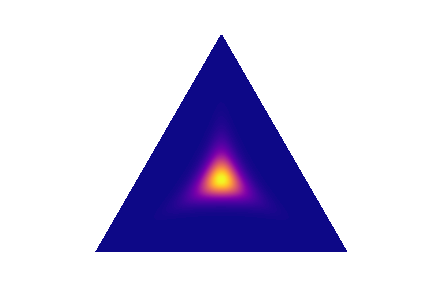
\includegraphics[width=\textwidth]{plots/notebooks/gs5.png}
\subcaption{}
\end{minipage}
\hfill
 \begin{minipage}[t]{.2\textwidth}
   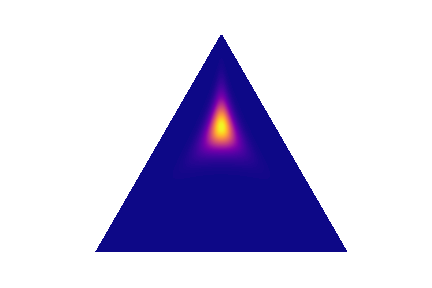
\includegraphics[width=\textwidth]{plots/notebooks/gs5_shift.png}
\subcaption{}
\end{minipage}

\caption{Пример распределения Gumbel-Softmax при различных значениях параметров: а)~$\lamT\to0$, б)~$\lamT=1, \s=[1,1,1]$, в)~$\lamT=5, \s=[1,1,1]$, г)~$\lamT=5, \mathbf{s}=[10,0.1,0.1].$}
\label{fig:gs}

\end{figure}


Заметим, что предлагаемое априорное распределение неоднозначно: одно и то же распределение  можно получить с различными значениями гиперпараметра $\mathbf{A}^{j,k}_l$ и структурного параметра $\gamma^{j,k}_l$. В качестве регуляризатора для матрицы $(\mathbf{A}^{j,k}_l)^{-1}$ предлагается использовать обратное гамма-распределение:
\[
    (\A^{j,k}_l)^{-1} \sim \text{inv-gamma}(\lambda_1,\lambda_2),
\]
где $\lambda_1,\lambda_2 \in \lam$ --- метапараметры оптимизации. 
Использование обратного гамма-распределения в качестве распределения гиперпараметров можно найти в~\cite{bishop,mackay}. В данной работе обратное распределение выступает как регуляризатор гиперпараметров.
Варьированием метапараметров $\lambda_1,\lambda_2$ получается  более сильная или более слабая регуляризация~\cite{rvm}. Пример распределений $\text{inv-gamma}(\lambda_1,\lambda_2)$ для разных значений метапараметров $\lambda_1,\lambda_2$ изображен на Рис.~\ref{fig:inv-gamma}. Оптимизации без регуляризации соответствует случай предельного распределения $\lim_{\lambda_1,\lambda_2\to 0}\text{inv-gamma}(\lambda_1, \lambda_2)$.

\begin{figure}
\centering
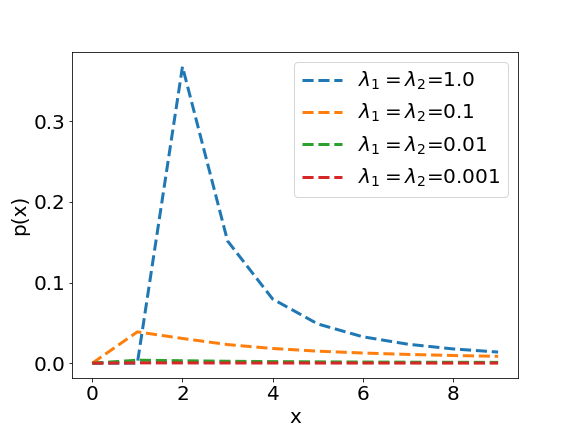
\includegraphics[width=0.6\textwidth]{plots/notebooks/invgamma.png}
\caption{Графики обратных гамма распределений для различных значений метапараметров.}
\label{fig:inv-gamma}
\end{figure}


Таким образом, предлагаемая вероятностная модель содержит следующие компоненты:
\begin{enumerate}
\item Параметры $\w$ модели, распределенные нормально.
\item Структура модели $\G$, содержащая все структурные параметры $\{\g^{j,k}, (j,k) \in E\}$, распределенные по распределению Gumbel-Softmax.
\item Гиперпараметры $\h = [\text{diag}(\A), \s]$, где $\A$ --- конкатенация матриц $\A^{j,k}, (j,k) \in E,$ $\s$ --- конкатенация параметров Gumbel-Softmax распределений $\s^{j,k}, (j,k) \in E$, где $E$ --- множество ребер, соответствующих графу рассматриваемого параметрического семейства моделей $\F$.
\item Метапараметры: $\lam = [\lambda_1, \lambda_2, \lamT].$ Эти параметры не подлежат оптимизации и задаются экспертно. 
\end{enumerate}

График вероятностной модели в формате плоских нотаций представлен на Рис.~\ref{fig:plate_prob}.
\begin{figure}
\centering
   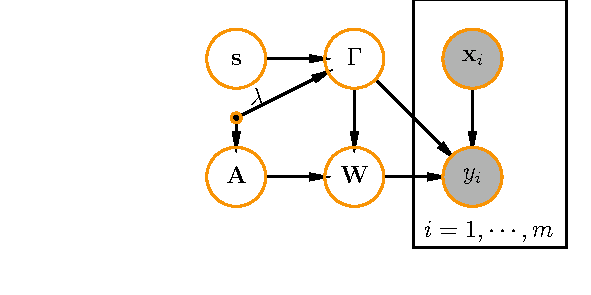
\includegraphics[width=0.5\textwidth]{plots/notebooks/simple_plate.pdf}
\caption{График предлагаемой вероятностной модели в формате плоских нотаций. Переменные обозначены белыми и серыми кругами, константы обозначены обведенными черными кругами. Наблюдаемые переменные обозначены серыми кругами.}
\label{fig:plate_prob}
\end{figure}

\section{Вариационная оценка обоснованности вероятностной модели}
Задача выбора структуры $\G$ и параметров $\w$ заключается в получении оценок на апостериорное распределение $\post = \postG\postw$. Оно зависит от гиперпараметров $\h$. 
В качестве критерия выбора гиперпараметров предлагается использовать апостериорную вероятность гиперпараметров:
\begin{equation}
\label{eq:optimal_hyper}
    \posth \propto \EV \priorh \to \max_{\h \in \Hb}.
\end{equation}
Структура модели и параметры модели выбираются на основе полученных значений гиперпараметров:
\[
    \w^*,\G^* = \argmax_{\w \in \Wb, \G \in \Gb} p(\w, \G|\y, \X, \h^*, \lam ),
\]
где $\h^*$ --- решение задачи оптимизации~\eqref{eq:optimal_hyper}.

Для вычисления обоснованности модели $$\EV = \iint_{\G, \w}\LL \priorw \priorG d\G d\w$$ из~\eqref{eq:optimal_hyper} предлагается использовать нижнюю вариационную оценку обоснованности.

\begin{theorem}
Пусть $\q = \qw \qG$ --- вариационное распределение c параметрами $\teta= [\tetaw, \tetaG ]$, аппроксимирующее апостериорное распределение структуры и параметров:
\[
    \q \approx \post,
\]
\[
    \qw  \approx \postw,
\]
\[
    \qG \approx \postG.
\]

Тогда справедлива следующая оценка:
\begin{equation}
\label{eq:full_elbo}
\log \EV \geq
\end{equation}
\[
 \E_{\q}  \log \LL - \KL{\qG}{\priorG} - 
\]
\[
 - \KL{\qw}{\priorw},
\]
где $\KL{\qw}{\priorw}$ вычисляется по формуле условной дивергенции:
\[
\KL{\qw}{\priorw} = \E_{\G \sim \qG} \E_{\w \sim \qw} \log \left(\frac{\qw}{\priorw}\right).
\]
\end{theorem}

\begin{proof}
Перепишем обоснованность:
\[
\log \EV  =  \log \iint_{\G,\w} \LL \priorw \priorG d\G d\w  =
\]
\[
   = \log\iint_{\G,\w} \LL \prior  \frac{\q}{\q}d\G d\w =
\]
\[
  =  \log \E_{\q} \frac{\LL \prior}{\q}.
\]
Используя неравенство Йенсена получим 
\[
 \log \E_{\q} \frac{\LL \prior}{\q} \geq  \E_{\q}\log \frac{\LL \prior}{\q} = 
\]
\[
 =  \E_{\q} \log \LL - \KL{\q}{\prior}.
\]
Декомпозируем распределение $q$ по свойству условной дивергенции:
\[
\KL{\q}{\prior} = 
\]
\begin{equation}
\label{eq:kl_full}
= \KL{\qG}{\priorG} + \E_{\G \sim \qG} \E_{\w \sim \qw} \log \left(\frac{\qw}{\priorw}\right).    
\end{equation}
\end{proof}
В качестве вариационного распределения $\qw$ предлагается использовать нормальное распределение, не зависящее от структуры модели $\G$:
\[
    \qw  \sim \mathcal{N}(\boldsymbol{\mu}_q, \A_q^{-1}), 
\]
где $\A_q^{-1}$ --- диагональная матрица с диагональю $\boldsymbol{\alpha}_q$.

В качестве вариационного распределения $\qG$ предлагается использовать произведение распределений Gumbel-Softmax. Конкатенацию параметров концентрации распределений обозначим $\s_q$. Его температуру, общую для всех структурных параметров $\g \in \G$, обозначим $\theta_\text{temp}$.
Вариационными параметрами распределения $\q$ являются параметры распределений $\qw, \qG$:
\[\teta =[\boldsymbol{\mu}_q, \boldsymbol{\alpha}_q,\s_q, \theta_\text{temp}]. 
\]
График вероятностной вариационной модели в формате плоских нотаций представлен на Рис.~\ref{fig:plate_qprob}.
\begin{figure}
\centering
   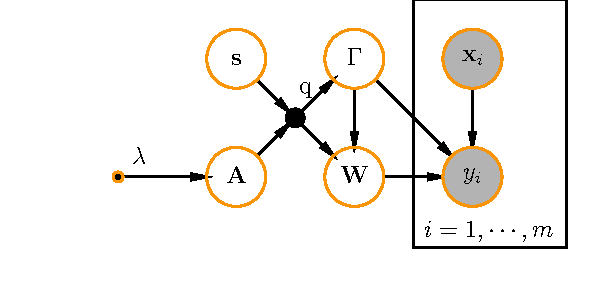
\includegraphics[width=0.5\textwidth]{plots/notebooks/plate.pdf}
\caption{График предлагаемой вероятностной вариационной модели в формате плоских нотаций. Переменные обозначены белыми и серыми кругами, константы обозначены обведенными черными кругами. Вариационное распределение обозначено черным кругом. Наблюдаемые переменные обозначены серыми кругами.}
\label{fig:plate_qprob}
\end{figure}
Для анализа сложности полученной модели введем понятие \textit{параметрической сложности}. 
\begin{defin} 
Параметрической сложностью  $C_p(\teta|\Uh, \lam)$ модели с вариационными параметрами $\teta$ на компакте $\Uh \subset \Hb$ назовем минимальную дивергенцию между вариационным и априорным распределением:
\[
C_p(\teta|\Uh, \lam) = \min_{\h \in \Uh} \KL{\q}{\prior}.
\]
\end{defin}
Параметрическая сложность модели соответствует минимальной по $\h \in \Uh$ минимальной ожидаемой длине описания параметров модели при условии заданного параметрического априорного распределения~\cite{hinton_mdl}.

Одним из критериев удаления неинформативных параметров в вероятностных моделях является отношение вариационной плотности параметров в моде распределения к вариационной плотности параметра в нуле~\eqref{eq:rho_graves}:
\[\frac{\qw[w=\mu_q]}{\qw[w=0]}= \text{exp}\left(-\frac{\alpha_q^2}{2\mu_q^2}\right),
\]
где параметру модели $w$ соответствуют вариационные параметры $\mu_q, \alpha_q$: $\qw[w] \sim \mathcal{N}(\mu_q, \alpha_q).$

Обобщим понятие относительной вариационной плотности на случай произвольных непрерывных распределений.
\begin{defin}
Относительной вариационной   плотностью параметра $w \in \w$  при условии структуры $\G$ и гиперпараметров $\h$ назовем отношение вариационной плотности в моде вариационного распределения параметра к вариационной плотности в моде априорного распределения параметра:
\[
\rho(w|\G,\tetaw, \h,\lam)=\frac{\qw[\text{mode}~\qw[w]]}{\qw[\text{mode}~{\priorw[w]}]}.
\]
Относительной вариационной плотностью вектора параметров $\mathbf{w}$ назовем следующее выражение:
\[
    {\rho}(\w|\G, \tetaw, \h,\lam) = \prod_{w \in \w}\rho(w|\G,\tetaw,\h,\lam).
\]

\end{defin}

Сформулируем и докажем теорему о связи относительной плотности и параметрической сложности модели. Предварительно докажем две вспомогательные леммы.

\begin{lemma}
\label{lem:cp_bound}
Пусть
\begin{enumerate}

\item Заданы компактные множества $\Uh \subset \Hb, \Utetaw \subset \Tetawb, \UtetaG \subset \TetaGb$.

\item Вариационное распределение $\qw$  является абсолютно непрерывным и унимодальным на  $U_{\boldsymbol{\theta}}$.
Его мода и матожидание совпадают:

\[
  \text{mode}~\qw = \E_{\qw} \w.
\]




\item Априорное распределение $\priorw$ является абсолютно непрерывным и унимодальным на  $U_\mathbf{h}$. Его мода и матожидание совпадают и не зависит от гиперпараметров $\h$  на $\Uh$ и структуры $\G$ на $\UtetaG$:
\[
\E_{\priorw}~\w = \text{mode}~\priorw[][\G_1][\h_1]=\text{mode}~\priorw[][\G_1][\h_2]=\mathbf{m}
\]
\text{ для любых }$~\h_1,\h_2 \in \Uh, \G_1,\G_2 \in \UG$.


\item Параметры модели $\w$ имеют конечные вторые моменты по маргинальным распределениям:
\[
   \int_{\G}\qG\qw d\G, \quad \int_{\G}\qG\priorw d\G.
\]


\item Вариационное распределение $\qw$ является липшецевым по $\w$.

\item Значение $\qw[\mathbf{m}]$ не равно нулю при $\teta \in \Uteta$.
\end{enumerate}
Тогда 
\[
   \left|\E_{\qG} {\rho}(\w|\G, \tetaw, \h, \lam) - 1\right| \leq
\]
\[
\leq \frac{C_l}{\min_{\Gamma \in \Gb, \tetaw \in \Uteta} \qw[\mathbf{m}]} \iint_{\G,\w} |\w| \cdot |\qw - \priorw|\qG d\w d\G,
\]
где $C_l$ --- максимальная константа Липшица для $\qw$ на $\Uteta$.

\end{lemma}
\begin{proof}
Для произвольного $\teta=[\tetaw, \tetaG]$ рассмотрим выражение:
\[
   \left|\E_{\qG} {\rho}(\w|\G, \tetaw, \h, \lam) - 1\right| =
\]
\[
   \left|\int_{\G} \left(\frac{\qw[\text{mode}~\qw]}{\qw[\text{mode}~\priorw]} \right)\qG d\G  - 1 \right| =
\]
\textit{представляя единицу как дробь с равными знаменателем и числителем}
\begin{multline*}
\hspace{-1cm}
 =  \bigl|\int_{\G} \left(\frac{\qw[\text{mode}~\qw] - \qw[\text{mode}~\priorw]}{\qw[\text{mode}~\priorw]}\right) \qG d\G \bigr| =
\end{multline*}
\textit{заменяя моду на матожидание (по условию теоремы)}
\[  = \left|\int_{\G} \left( \frac{\qw[\E_{\qw}\w] - \qw[\E_{\priorw} \w]}{\qw[\mathbf{m}]}\right)  \qG d\G\right| \leq 
\]
\textit{занося модуль под знак интеграла}
\[
\leq 
\int_{\G} \left|\frac{\qw[\E_{\qw} \w)] - \qw[\E_{\priorw} \w]}{{\qw[\mathbf{m}]}} \qG d\G\right| \leq
\]
\textit{используя липшецевость функции }$\qw$
\[
\frac{C_l}{\min_{\Gamma \in \Gb, \tetaw \in \Uteta} \qw[\mathbf{m}]}\int_{\G}  |\E_{\qw}\w - \E_{\priorw}\w|\qG d\G  \leq
\]
\textit{расписывая матожидание через интеграл}
\[
    \leq \frac{C_l}{\min_{\tetaw \in \Uteta} \qw[\mathbf{m}]} \iint_{\G,\w} |\w| \cdot |\qw - \priorw|\qG d\w d\G,
\] 
что и требовалось доказать.
\end{proof}



\begin{lemma}
\label{lem:pinsk}
Пусть
\begin{enumerate}
\item Вариационное распределение $\qw$ и априорное распределение $\priorw$  являются абсолютно непрерывными.

\item Решение задачи 
\begin{equation}
\label{eq:dkl_solve}
\h^{*} = \argmin_{\h \in \Uh} \KL{\q}{\prior}
\end{equation} единственно для любого $\teta \in \Uteta$.



\item Задана  бесконечная последовательность векторов вариационных параметров $\teta[1],\teta[2],\dots,\teta[i],\dots \in \Uteta$, такая что $\lim_{i \to \infty}C_p(\teta[i]|\Uh,\lam) = 0.$
Тогда следующее выражение стремится к нулю:
\[
 \iint_{\w,\G} |\priorw[][][{\h[i]}] - \qw[][][{\tetaw[i]}]| \qG[][{\tetaG[i]}] d\G d\w,
\]
где $\teta[i] = \left[\tetaw[i], \tetaG[i]\right],$ $\h[i]$ --- решение задачи~\eqref{eq:dkl_solve} для $\teta[i]$.

\end{enumerate}
\end{lemma}
\begin{proof}
Воспользуемся неравенством Пинскера~\cite{pinsker}:
\[
    ||F_q(\tetaw[i])-F_p(\h[i])||_\text{TV}\leq\sqrt{\frac{1}{2}\widehat{\text{KL}}\left(\priorw[][][{\h[i]}]||\qw[][][{\tetaw[i]}]\right)},
\]
где $||\cdot||_\text{TV}$ --- расстояние по вариации, $F_q, F_p$ --- функции распределения  $\qw,\priorw,$  $\widehat{\text{KL}}\left(\priorw||\qw\right)$ --- дивергенция при фиксированной структуре $\G$:
\[
   \int_{\w} \qw \log \left(\frac{\qw}{\priorw}\right) d\w.
\]

По условию дивергенция~\eqref{eq:kl_full} стремится к нулю при $i \to \infty$. Она декомпозируется на два  неотрицательных слагаемых, поэтому оба они стремятся к нулю.
Рассмотрим второе слагаемое:
\[
  0 =   \lim_{i \to \infty} \E_{\G \sim \qG[][{\tetaG[i]}]} \E_{\w \sim \qw[][][{\tetaw[i]}]} \log \left(\frac{\qw[][][{\tetaw[i]}]}{\priorw[][][{\h[i]}]}\right) = 
\]
%\begin{center}
\textit{расписывая матожидание как интеграл}
%\end{center}
\[
 =  \lim_{i \to \infty} \left|\int_{\G} \int_{\w} \log \left(\frac{\qw[][][{\tetaw[i]}]}{\priorw[][][{\h[i]}]}\right)\qG[][{\tetaG[i]}]\qw[][][{\tetaw[i]}] d\w d\G \right| \geq  
\]
%\begin{center}
\textit{по неравенству Пинскера}
%\end{center}
\[
\geq \lim_{i \to \infty}  \int_{\G} ||F_q({\tetaw[i]})-F_p({\h[i]})||^2_\text{TV}\qG[][{\tetaG[i]}] d\G \geq 0.  
\]

Отсюда
\[
\lim_{i \to \infty}  \int_{\G} ||F_q({\tetaw[i]})-F_p({\h[i]})||^2_\text{TV}\qG[][{\tetaG[i]}] d\G = 0.
\]

По неравенству Йенсена 
\[
0 \leq  \left(\int_{\G} ||F_q({\tetaw[i]})-F_p({\h[i]})||_\text{TV}\qG[][{\tetaG[i]}] d\G\right)^2 \leq
\]
\[
 \leq   \int_{\G} ||F_q({\tetaw[i]})-F_p({\h[i]})||^2_\text{TV}\qG[][{\tetaG[i]}] d\G.
\]
Тогда по свойству степени предела $$\lim_{i \to \infty} \int_{\G}||F_q({\tetaw[i]})-F_p({\h[i]})||_\text{TV} \qG[][{\tetaG[i]}] d\G = 0.$$
По лемме Шеффе~\cite{scheffe} TODO данное выражение можно переписать как:
\begin{equation}
\label{eq:sheffe}
    \lim_{i \to \infty}   \frac{1}{2}\iint_{\w,\G} |\priorw[][][{\h[i]}] - \qw[][][{\tetaw[i]}]| \qG[][{\tetaG[i]}] d\G d\w = 0,
\end{equation}
что и требовалось доказать.
\end{proof}




\begin{theorem}
Пусть выполнены условия Леммы~\ref{lem:cp_bound} и  Леммы~\ref{lem:pinsk}.
Тогда справедливо следующее выражение:
\[
   \lim_{i \to \infty} \E_{\qG[][{\tetaG[i]}]} {\rho}(\w|\G, {\tetaw[i]}, {\h[i]}, \lam) = 1.
\]

\end{theorem}

\begin{proof}

По Лемме 2
\[
    \E_{\qG[][{\tetaG}]} {\rho}(\w|\G, {\tetaw}, {\h}, \lam)  \leq
\]
\[
\leq  \frac{C_l}{\min_{\G in \Gb, \tetaw \in \Uteta} \qw[\mathbf{m}]}  \iint_{\G,\w} |\w| \cdot |\qw - \priorw|\qG d\w d\G.
\]

%https://math.stackexchange.com/questions/112786/convergence-in-law-and-uniformly-integrability
Докажем что величина
\[
    \iint_{\G,\w} |\w| \cdot |\qw - \priorw|\qG d\w d\G
\]
стремится к нулю.
Определим случайную величину $\boldsymbol{\nu}(t), t \geq 0$ следующим образом:
\[
    \boldsymbol{\nu}(t) = \boldsymbol{\max}(-t \cdot \mathbf{1}, \boldsymbol{\min}(t \cdot \mathbf{1}, \w)).
\]
Данная величина совпадает с $\w$ при $|\w| < t$ и принимает значение $t$ или $-t$ при $|\w| \geq t.$
Тогда для любого $t>0$ справедливо:
\[
    \iint_{\G,\w} |\w| \cdot |\qw - \priorw|\qG d\w d\G \leq
\]
\textit{по неравенству треугольника и используя выражение }$\w = \w + \boldsymbol{\nu}(t) -\boldsymbol{\nu}(t)$
\begin{equation}
\label{eq:tmp}
    \leq    \iint_{\G,\w} |\w -\boldsymbol{\nu}(t)| \cdot |\priorw -\qw|\qG d\w d\G   +
\end{equation}
\[ +      \iint_{\G,\w} |\boldsymbol{\nu}(t)| \cdot |\qw - \priorw|\qG d\w d\G.
\]




Рассмотрим первое слагаемое суммы~\eqref{eq:tmp}. Т.к. вторые моменты $\E_{\qG}\E_{\qw} \w^2, \E_{\qG}\E_{\priorw} \w^2$ конечны, то случайная величина $\w$ равномерно интегрируема как при маргинальном распределении $\int_{\G}\qG\qw d\G$, так и при маргинальном распределении $\int_{\G}\qG\priorw d\G$.
По определению равномерной интегрируемости для $\w$ для любого числа $\varepsilon$ существует число $t_0$, такое что для любого $t \geq t_0$, любого $\h \in \Uh, \teta \in \Uteta$,  справедливо выражение:
\[
    \E_{\qG}\E_{\qw}|\w - \boldsymbol{\nu}(t)| = \iint_{\w,\G}|\w - \boldsymbol{\nu}(t)|\qw\qG d\w d\G \leq \varepsilon,
\]
\[
    \E_{\qG}\E_{\priorw}|\w - \boldsymbol{\nu}(t)| = \iint_{\w,\G}|\w - \boldsymbol{\nu}(t)|\priorw\qG d\w d\G \leq \varepsilon.
\]
Тогда
\[
   \iint_{\G,\w} |\w -\boldsymbol{\nu}(t)|\cdot|\priorw  - \qw| d\w d\G   \leq  
\]
\textit{так как модуль разностей меньше или равен суммы модулей}
\[
  \iint_{\G,\w} |\w -\boldsymbol{\nu}(t)|\priorw  +   \iint_{\G,\w} |\w -\boldsymbol{\nu}(t)|\qw d\G d\w < 2 \varepsilon
\]
для любого $t \geq t_0$. Обозначим за $\varepsilon(t)$ минимальное число $\varepsilon$, удовлетворяющее предыдущим неравенствам. Тогда
$$
 \iint_{\G,\w} |\w -\boldsymbol{\nu}(t)|\cdot|\priorw  - \qw| d\w d\G  \leq 2 \varepsilon(t),
$$
где $\lim_{t \to \infty} \varepsilon(t) = 0$.

Рассмотрим второе слагаемое.
$$
\iint_{\G,\w} |\boldsymbol{\nu}(t)|\cdot |\qw - \priorw| d\w d\G \leq 
$$
\textit{по ограниченности функции }$\boldsymbol{\nu}(t)$
$$
  \leq  t \iint_{\G,\w}  |\qw - \priorw|\qG d\w d\G.
$$

Переходя к пределу в ~\eqref{eq:tmp} получим:
$$
    \lim_{i \to \infty} \iint_{\G,\w} |\w| \cdot |\qw - \priorw[][][{\h[i]}]|\qG[][{\tetaG[i]}] d\w d\G  =
$$
\textit{добавим предел по }$t$\textit{, от которого не зависит данное выражение}
$$
= \lim_{t \to \infty}\lim_{i \to \infty}\iint_{\G,\w} |\w|\cdot |\qw[][][{\tetaw[i]}] - \priorw[][][{\h[i]}]|\qG[][{\tetaG[i]}] d\w d\G \leq
$$
\textit{из выше написанных неравенств}
$$
    \lim_{t \to \infty}\lim_{i \to \infty} \iint_{\G,\w} |\w -\boldsymbol{\nu}(t)|\cdot|\priorw[][][{\h[i]}] -\qw[][][{\tetaw[i]}]| d\w d\G   +
$$
$$
 + \iint_{\G,\w} |\boldsymbol{\nu}(t)| \cdot |\qw[][][{\tetaw[i]}] - \priorw[][][{\h[i]}]|\qG[][{\tetaG[i]}] d\w d\G \leq
$$
$$
     \lim_{t \to \infty}  2\varepsilon(t)  + \lim_{t \to \infty}\lim_{i \to \infty}  t \iint_{\G,\w}  |\qw[][][{\tetaw[i]}] - \priorw[][][\h_i]\qG[][{\tetaG[i]}] = 0.
$$
Последнее равенство следует из Леммы~\ref{lem:pinsk}.
Таким образом выражение $$\left|\int_{\G} \frac{\qw[\text{mode}\qw]}{\qw[\text{mode}\priorw]}\qG d\G \right|$$ стремится к единице, что и требовалось доказать.
\end{proof}

Теорема утверждает, что при устремлении параметрической сложности модели к нулю, все параметры $\w$  модели подлежат удалению в среднем по всем возможным значениям  структуры $\G$ модели. Заметим, что теорема применима для случая, когда последовательность вариационных распределений $\q$ не имеет предела. Так, в случае, если структура $\G$ определена однозначно, последовательность $\teta_i$ может являться последовательностью нормальных распределений, чье матожидание стремится к нулю:
\[
    \teta_i \sim \mathcal{N}(\boldsymbol{\mu}_q[i], \A^{-1}_q[i]), \boldsymbol{\mu}_q[i] \to \mathbf{0}.
\]
Априорным распределением $\prior = \priorw$ при этом может являться семейство нормальных распределений с нулевым средним:
\[
    \priorw = \mathcal{N}(\mathbf{0}, \A^{-1}).
\]
При этом сама последовательность распределений $\teta[i]$ не обязана иметь предел.

\section{Обобщающая задача}
В данном разделе проводится анализ основных критериев выбора моделей, а также предлагается их обобщение на случай моделей, испольюзующих вариационное распределение $\q$ для аппроксимации неизвестного апостериорного распределения параметров $\prior$.

Рассмотрим основные статистические критерии выбора вероятностных моделей. 
\begin{enumerate}
\item Критерий максимального правдоподобия:
\[\log \LL \to \max_{\w \in \Uw, \G \in \UG}.\]
Для использования данного критерия в качестве задачи выбора модели предлагается следующее обобщение:
\begin{equation}
\label{eq:optim_ml}
    \Loss =  \E_{\q} \log~\LL.
\end{equation}
Данное обобщение~\eqref{eq:optim_ml} эквивалентно  критерию максимального правдоподобия при выборе в качестве $\q$ эмпирического распределения параметров TODO и структуры.
Метод не предполагает оптимизации гиперпараметров $\h$. Для формального соответствия данной задачи задаче выбора модели~\eqref{eq:optim_problem},\eqref{eq:optim_problem_in}, т.е. двухуровневой задачи оптимизации, положим $\Loss=\Val:$
\[
    \Loss =  \E_{\q}\log \LL \to \max_{\teta \in \Uteta},
\]
\[
    \Val =  \E_{\q}\log \LL \to \max_{\h \in \Uh}.
\]



\item Метод максимальной апостериорной вероятности. 
\[\log \LL \prior \to \max_{\w  \in \Uw, \G \in \UG}.\]
Аналогично предыдущему методу сформулируем вариационное обобщение данной задачи:
\begin{equation}
\label{eq:optim_map}
\Loss = \Val = 
\end{equation}
\[
 = \E_{\q} \bigl( \log\LL + \log\prior \bigr).
\]
Т.к. в рамках данной задачи~\eqref{eq:optim_map} не предполагается оптимизации гиперпараметров $\h$, положим параметры распределения $\prior$ фиксированными:
\[
   \lam = [\lambda_1, \lambda_2, \lamT, \s, \text{diag}(\A)].
\]

\item Полный перебор структуры:
\begin{equation}
\label{eq:optim_struct}
    \Loss = \Val = \E_{\q} \log \LL [\qG = p']
\end{equation}
где $p'$ --- некоторое распределение на структуре $\G$, выступающее в качестве метапараметра.




\item Критерий Акаике:
\[
   \text{AIC} =  \log \LL - |\Wb|.
\]
Т.к. все рассматриваемые модели принадлежат одному параметрическому семейству моделей $\F$, то количество параметров у всех рассматриваемых моделей  совпадает. Тогда критерий Акаике совпадает с критерием максимального правдоподобия. Для использования критерия Акаике для сравнения моделей, принадлежащих одному параметрическому семейству~$\F$ предлагается следующая переформулировка:
\begin{equation}
\label{eq:optim_aic}
    \Loss = \Val = \log \LL - 
\end{equation}
\[
 - |\{w: \KL{\q}{\prior}<\lambda_\text{prune}\}|,
\]
где 
\begin{equation}\label{eq:aic_compl}\h=\argmin_{\h' \in \Uh} \KL{\q}{\prior},\end{equation} $\lambda_{\text{prune}}$ --- метапараметр алгоритма, $\Uh  \subset \Hb$ --- область определения задачи по гиперпараметрам. Предложенное обобщение~\eqref{eq:optim_aic} применимо только в случае, если выражение~\eqref{eq:aic_compl} определено однозначно, т.е. существует единственный вектор гиперпараметров  $\h \in \Uh,$ доставляющий минимум дивергенции $\KL{\q}{\prior}.$

\item Информационный критерий Шварца:
\[
    \text{BIC} = \log \LL -0.5\log m|\Wb|.
\]
Переформулируем данный критерий аналогично критерию AIC:
\begin{equation}
\label{eq:optim_bic}
    \Loss = \Val =  
\end{equation}
\[
\log \LL - 0.5 \log m |\{w: \KL{\q}{\prior}<\lambda_{\text{prune}}\}|,
\]
метапараметр $\lambda_{\text{prune}}$ определен аналогично~\eqref{eq:aic_compl}.

\item Метод вариационной оценки обоснованности:
\begin{equation}
\label{eq:optim_elbo_method}   
    \Loss = 
\end{equation}
\[
= \E_{\q} \log \LL - \KL{\q}{\prior} + 
\]
\[
+\log\priorh \to \max_{\teta \in \Uteta},
\]
\[
     \Val = 
\]
\[
= \E_{\q} \log \LL - \KL{\q}{\prior} +
\]
\[+ \log\priorh \to \max_{\h \in \Uh},
\]
В рамках данной задачи функции $\Loss$ и $\Val$ совпадают, все гиперпараметры $\h$ подлежат оптимизации.

\item Валидация на отложенной выборке:
\begin{equation}
\label{eq:optim_hold_out}
    \Loss = \E_{\q} \log \LL[\y_\text{train}][\X_\text{train}] + \log \prior \to \max_{\teta \in \Uteta},
\end{equation}
\[
    \Val = \E_{\q} \log \LL[\X_\text{test}][\y_\text{test}] \to \max_{\h \in \Uh},
\]
где $(\X_\text{train}, \y_\text{train}), (\X_\text{test}, \y_\text{test})$ --- разбиение выборки на обучающую и контрольную подвыборку.
В рамках данной задачи, все гиперпараметры $\h$ подлежат оптимизации.

\end{enumerate}

Каждый из рассмотренных критериев удовлетворяет хотя бы одному из перечисленных свойств:
\begin{enumerate}[label={\arabic*)}]
\item модель, оптимизируемая согласно критерию, доставляет максимум правдоподобия выборки;
\item модель, оптимизируемая согласно критерию, доставляет максимум оценки обоснованности;
\item для моделей, доставляющих сопоставимые значения правдоподобия выборки, выбирается модель с меньшим количеством информативных параметров.
\item критерий позволяет производить перебор структур для отбора наилучших.
\end{enumerate}

Формализуем рассмотренные критерии. Оптимизационную задачу, которая удовлетворяет всем перечисленным свойствам при некоторых значинях метапараметров, будет называть \textit{обобщающей}.

\begin{defin}
Двухуровневую задачу оптимизации будем называть \textit{обобщающей} на компакте $$U = \Utetaw \times \UtetaG \times \Uh \times \Ulam \subset \Tetawb \times \TetaGb \times \Hb \times \Lamb,$$ если она удовлетворяет следующим критериям.
\begin{enumerate}
\item Область определения каждого параметра $w \in \w$, гиперпараметра $h \in \h$ и метапараметра $\lambda \in \lam$ не  является пустым множеством и не является точкой.
\item Для каждого значения гиперпараметров $\h$ оптимальное решение нижней задачи оптимизации~\eqref{eq:optim_problem_in} 
\[
\teta^{*}(\h) = \argmax_{\teta \in \Tetab} \Loss
\]
определено однозначно при любых значениях метапараметров $\lam \in \Ulam$.

\item Критерий максимизации правдоподобия выборки: существует $\lam \in \Ulam$ и  $K_1>0$,$$K_1 < \max_{\h_1,\h_2 \in \Uh} \Val[\h_1][][][\teta^{*}(\h_1)] - \Val[\h_2][][][\teta^{*}(\h_2)],$$ такие что для любых векторов гиперпараметров $\h_1, \h_2 \in \Uh,$ удовлетворяющих неравенству $$\Val[\h_1][][][\teta^{*}(\h_1)] - \Val[\h_2][][][\teta^{*}(\h_2)] > K_1,$$ выполняется неравенство $$\E_{\q[\teta^{*}(\h_1)]}\log\LL > \E_{\q[\teta^{*}(\h_2)]}\log\LL.$$

\item Критерий минимизации параметрической сложности:  существует  $\lam \in \Ulam$ и $K_2>0,$ $$K_2 < \max_{\h_1, \h_2 \in \Uh} \Val[\h_1][][][\teta^{*}(\h_1)] - \Val[\h_2][][][\teta^{*}(\h_2)],$$ такие что для любых векторов гиперпараметров $\h_1,\h_2 \in \Uh$, удовлетворяющих неравенству $$\Val[\h_1][][][\teta^{*}(\h_1)] - \Val[\h_2][][][\teta^{*}(\h_2)]>K_2,$$ параметрическая сложность первой модели меньше, чем второй: $$C_p(\teta^{*}(\h_1)|\Uh,\lam)<C_p(\teta^{*}(h_2)|\Uh,\lam).$$

\item Критерий приближения оценки обоснованности: существует значение гиперпараметров $\lam$, такое что значение функций потерь $\Val$ как сложной функции от $\Loss$ пропорционально вариационной оценки обоснованности модели: $$\Val[][][][\teta^{*}(\h)] \propto $$
$$\propto
\E_{\q[\teta'(\h)]}\log\LL - \KL{\q[\teta'(\h)]}{\prior} + \log\priorh$$ для всех $\h \in \Uh,$
где в качестве гиперпараметров $\h$ рассматриваются все гиперпараметры модели, вне зависимости от критерия и особенности его оптимизации гиперпараметров: $$\h = [\A, \s],$$
где $$\teta'(\h) = \argmax_{\teta \in \Uh} \E_{\q[\teta]}\log\LL - \KL{\q[\teta]}{\prior}.$$

\item Критерий перебора оптимальных структур: существует константа $K_3>0$, такая что существует хотя бы одна пара гиперпараметров $\h_1, \h_2 \in \Uh,$ удовлетворяющая неравенствам:
$$\KL{\priorG[][\h_1]}{\priorG[][\h_2]} > K_3,\KL{\priorG[][\h_2]}{\priorG[][\h_1]}>K_3$$ и набор метапараметров $\lam$, такие что для произвольных локальных оптимумов  $\h_1,\h_2$ задачи оптимизации $\Val$, полученных при метапараметрах $\lam$ и удовлетворяющих неравенствам $$\KL{\priorG[][\h_1]}{\priorG[][\h_2]} > K_3, \KL{\priorG[][\h_2]}{\priorG[][\h_1]}>K_3,$$$$\Val[\h_1] > \Val[\h_2],$$  существует значение метапараметров $\lam' \neq \lam$, такие что
\begin{enumerate}
\item соответствие между вариационными параметрами $\teta^{*}(\h_1),\teta^{*}(\h_2)$ сохраняется при  $\lam'$,
\item выполняется неравенство $\Val[\h_1][][][][\lam'] < \Val[\h_2][][][][\lam']$.
\end{enumerate}


\item Критерий нерперывности: функции $\Loss$ и $\Val$ непрерывны по метапараметрам $\lam \in \Ulam$.
\end{enumerate}
\end{defin}
Первый критерий является техническим и используется для исключения из рассмотрения вырожденных задач оптимизации.  
Второй критерий говорит о том, что решение первого и второго уровня должны быть согласованы и определены однозначно.
Критерии 3-5 определяют возможные критерии оптимизации, которые должны приближаться обобщающей задачей.
Критерий 6 говорит о возможности перехода между различными структурами модели. Данный критерий говорит о том, что мы можем перейти от одного набора гиперпараметров $\h_1$ к другим $\h_2$, если они соответствуют локальным оптимумам задачи оптимизации, и дивергенция соответствующих априорных  распределений на структурах $\priorG$ значимо высока. При этом соответствующие вариационные распределения $\qG$ могут оказаться достаточно близки, несмотря на значимые различия априорных распределений. Поэтому возможным дополнением этого критерия был бы критерий, позволяющий переходить от структуры к структуре, если соответствующие распределения $\qG$ различаются значимо.
Последний критерий говорит о том, что обобщающая задача должна позволять производить переход между различными методами выбора  параметров и структуры модели непрерывно.

\begin{theorem}Рассмотренные задачи~\eqref{eq:optim_ml},\eqref{eq:optim_map},\eqref{eq:optim_struct},\eqref{eq:optim_aic},\eqref{eq:optim_bic},\eqref{eq:optim_hold_out} не являются обобщающими.
\end{theorem}
\begin{proof}
Задачи~\eqref{eq:optim_ml},\eqref{eq:optim_map},\eqref{eq:optim_struct},\eqref{eq:optim_aic},\eqref{eq:optim_bic} не имеют гиперпараметров $\mathbf{h}$, подлежащих оптимизации, поэтому не могут приближать вариационную оценку.

При  использовании валидации на отложенной выборки~\eqref{eq:optim_hold_out} в функцию валидации $\Val$ не входит ни один метапараметр, поэтому критерий перебора структур 6 для нее также не выполняется. 
\end{proof}

Докажем также, что задача~\eqref{eq:optim_elbo_method} также не является обобщающей.
\begin{theorem}
Пусть $q_{\boldsymbol{\Gamma}}$ --- абсолютно непрерывное распределение с дифференцируемой плотностью, такой что:
\begin{enumerate}
\item Градиент плотности $\nabla_{\boldsymbol{\theta}_{\boldsymbol{\Gamma}}} q(\boldsymbol{\Gamma}|\boldsymbol{\theta}_{\boldsymbol{\Gamma}})$ является нулевым не более чем счетное количество раз. 
\item Выражение $\nabla_{\boldsymbol{\theta}_{\boldsymbol{\Gamma}}} q(\boldsymbol{\Gamma}|\boldsymbol{\theta}_{\boldsymbol{\Gamma}}) \text{log}p(\boldsymbol{\Gamma}|\mathbf{h}, \boldsymbol{\lambda})$ ограничено на $U_{\boldsymbol{\theta}}$ некоторой случайной величиной с конечным первым моментом.
\end{enumerate}
Тогда задача~\eqref{eq:optim_elbo_method} не является обобщающей.
\end{theorem}
\begin{proof}
Пусть выполнены условия критерия 6 о переборе структур, и $\mathbf{h}_1, \mathbf{h}_2$ --- локальные оптимумы функции $\Val$ при метапараметрах $\boldsymbol{\lambda}$.
По условию критерия соответствтие $\teta_1 = \boldsymbol{\theta}^{*}(\mathbf{h}_1)$ и $\teta_2 = \boldsymbol{\theta}^{*}(\mathbf{h}_2)$ должны сохраняться, т.е. для некоторого $\boldsymbol{\lambda}'$ решение  нижней задачи оптимизации $\boldsymbol{\theta}^{*}(\mathbf{h}_1)$ должно совпадать с решением $\boldsymbol{\theta}^{*}(\mathbf{h}_1)$ при метапараметрах $\boldsymbol{\lambda}$. Тогда
\[
  0 =  \nabla_{\boldsymbol{\theta}} \mathsf{E}_{q(\mathbf{w}, \boldsymbol{\Gamma}|\boldsymbol{\theta}_1)} \text{log}~p(\mathbf{y}|\mathbf{X}, \mathbf{w}, \boldsymbol{\Gamma}) -\nabla_{\boldsymbol{\theta}}  \text{D}_{\text{KL}}(q(\mathbf{w}, \boldsymbol{\Gamma}|\boldsymbol{\theta}_1) | p(\mathbf{w}, \boldsymbol{\Gamma}|\mathbf{h}_1, \boldsymbol{\lambda})) = 
\]
\[
= \nabla_{\boldsymbol{\theta}} \mathsf{E}_{q(\mathbf{w}, \boldsymbol{\Gamma}|\boldsymbol{\theta}_1)} \text{log}~p(\mathbf{y}|\mathbf{X}, \mathbf{w}, \boldsymbol{\Gamma}) - \nabla_{\boldsymbol{\theta}}  \text{D}_{\text{KL}}(q(\mathbf{w}, \boldsymbol{\Gamma}|\boldsymbol{\theta}_1) | p(\mathbf{w}, \boldsymbol{\Gamma}|\mathbf{h}_1, \boldsymbol{\lambda}')).
\]
Сокращая равные слагаемые в равенстве получим:
\[
\nabla_{\boldsymbol{\theta}}  \text{D}_{\text{KL}}(q(\boldsymbol{\Gamma}|\boldsymbol{\theta}_1) | p(\boldsymbol{\Gamma}| \boldsymbol{\lambda})) = \nabla_{\boldsymbol{\theta}} \text{D}_{\text{KL}}(q(\boldsymbol{\Gamma}|\boldsymbol{\theta}_1) | p(\boldsymbol{\Gamma}| \boldsymbol{\lambda}')),
\] 
Из второго условия теоремы следует, что по теореме Лебега о мажорируемой сходимости осуществим переход дифференцирования под знак интеграла:
\[
\int_{\boldsymbol{\Gamma} \in \amsmathbb{\Gamma}} \nabla_{\boldsymbol{\theta}_\Gamma} q(\boldsymbol{\Gamma}|\boldsymbol{\theta}_1) (\text{log}~p(\boldsymbol{\Gamma}| \boldsymbol{\lambda}) - \text{log}~p(\boldsymbol{\Gamma}| \boldsymbol{\lambda}')) d\boldsymbol{\Gamma} = 0.
\]
Т.к. выражение $ \nabla_{\boldsymbol{\theta}_\Gamma} q(\boldsymbol{\Gamma}|\boldsymbol{\theta}_1)$ принимает нулевое значение в счетном количестве точек, то выражение $\text{log}~p(\boldsymbol{\Gamma}| \boldsymbol{\lambda}) - \text{log}~p(\boldsymbol{\Gamma}| \boldsymbol{\lambda}')$ равно нулю почти всюду, что означает что метапараметр температуры $\lambda_\text{temp}$  равен при разных значениях метапараметров:
\[
\lambda_\text{temp} = \lambda_\text{temp}',\quad \lambda_\text{temp} \in \boldsymbol{\lambda}, \lambda_\text{temp}' \in \boldsymbol{\lambda}'.
\]
Таким образом, метапараметры $\boldsymbol{\lambda},\boldsymbol{\lambda}'$ отличаются лишь на метапараметры  $\lambda_1, \lambda_2$ регуляризации ковариационной матрицы~$\mathbf{A}^{-1}$. 
Возьмем в качестве векторов гиперпараметров $\mathbf{h}_1,\mathbf{h}_2$ гиперпараметры, отличающиеся только параметрами распределения структуры:
\[
    \mathbf{h}_1 = [\mathbf{s}_1, \text{diag}(\mathbf{A}_1)], \mathbf{h}_2 = [\mathbf{s}_2, \text{diag}(\mathbf{A}_2)],\quad \mathbf{s}_1 \neq \mathbf{s}_2, \mathbf{A}_1 = \mathbf{A}_2.
\]
Метапараметры $\lambda_1, \lambda_2$ не влияют на значение функции $\Val$ при гиперпараметрах, отличающихся только параметрами распределения структуры, поэтому значение функции $Q$ для них будет неизменно при любых значениях $\lambda_1, \lambda_2$. Приходим к противоречию: значение $\Val$ не меняется при изменении метапараметров $\boldsymbol{\lambda}$.

\end{proof}

В качестве обобщающей задачи оптимизации предлагается оптимизационную задачу следующего вида:
\begin{equation}
\label{eq:qopt}
\h^{*} = \argmax_{\h} \Val = 
\end{equation}
\[
= \lamLL \E_{\q[\teta^{*}]} \log\LL - 
\]
\[
    - \lamCQ \KL{\q[\teta^{*}]}{\prior} - 
\]
\[
    - \sum_{p' \in \mathfrak{P},\lambda \in \lamS} \lambda\KL{\q[\teta^{*}]}{p'} + \log\priorh, 
\]
\begin{equation}
\label{eq:lopt}
%\tag{$L^{*}$}
{\teta}^{*} = \argmax_{\teta} \Loss = 
\end{equation}
\[=
\E_{\q} \log \LL - \lamCL \KL{\q[\teta^{*}]}{\prior},
\]
где $\mathfrak{P}$ --- непустое множество распределений на структуре $\G$, $\lamCQ, \lamCL, \lamS$  --- некоторые числа. Множество распределений $\mathfrak{P}$ отвечает за перебор структур $\G$ в процессе оптимизации модели.
В предельном случае, когда температура $\lamT$ близка к нулю, а множество $\mathfrak{P}$ состоит из распределений, близких к дискретным, соответствующим всем возможным структурам, калибровка $\lamS$ порождает последовательность задач оптимизаций, схожую с перебором структур. Рассмотрим следующий пример. 

\begin{example} 
Рассмотрим вырожденный случай поведения функции $\Val$, когда $\lamLL = \lamCQ = 0$. Пусть модель использует один структурный параметр, в качестве априорного распределения на структуре задано распределение Gumbel-Softmax с $\lamT$. Пусть в качестве множества распределений $\mathfrak{P}$ используется два распределения Gumbel-Softmax, сконцентрированных близко к вершинам симплекса:
\[
    \mathfrak{P} = [\mathcal{GS}([0.95, 0.05, 0.05]^\text{T}, 1.0) ,\mathcal{GS}([0.95, 0.05, 0.05]^{\text{T}}, 1.0)].
\]

Из определения распределения Gumbel-Softmax следует, что достаточно рассмотреть только значения параметра $\mathbf{s}$ ,находящиеся внутри симплекса.
На рис.~\ref{fig:gs_comb} изображены значения функции Q в зависимости от метапараметров $\boldsymbol{\lambda}^\text{struct}_\text{Q}$ и значений гиперпараметра $\mathbf{s}$ распределения на структуре. Видно, что варьируя  коэффициенты метапараметров значение функции $\Val$ значительно меняется вблизи вершин симплекса. Таким образом получается последовательность оптимизаций, схожая с полным перебором структуры.
\end{example}


\begin{figure}
 \begin{minipage}[t]{.32\textwidth}
   \includegraphics[width=\textwidth]{plots/notebooks/struct_reg_1.png}
\subcaption{}
\end{minipage}
\hfill
 \begin{minipage}[t]{.32\textwidth}
   \includegraphics[width=\textwidth]{plots/notebooks/struct_reg_2.png}
\subcaption{}
\end{minipage}
\hfill
 \begin{minipage}[t]{.32\textwidth}
   \includegraphics[width=\textwidth]{plots/notebooks/struct_reg_3.png}
\subcaption{}
\end{minipage}

\caption{Пример зависимости функции $\Val$ от гиперпараметра $\s$ при различных значениях метапараметров $\lamS$. Темные точки на графике соответсвуют наименее предпочтительным значениям гиперпараметра. а)~$\lamS = [0,0],$ б)~$~\lamS = [1,0],$ в)~$~\lamS = [1,1].$}
\label{fig:gs_comb}

\end{figure}

Следующая теорема анализирует достаточные условия того, что предложенная задача оптимизации~\eqref{eq:qopt} является обобщающей.
\begin{theorem}
Пусть
\begin{enumerate}%[label={\arabic*)}] 
\item Задано непустое множество непрерывных по параметрам распределений на структуре $\mathfrak{P}$, чьи плотности не принимают нулевое значение, где хотя бы одно распределение $p_1 \in \mathfrak{P}$ является Gumbel-Softmax распределением, и для каждого значения $\s \in \Uh, \lamT \in \Ulam$ существует значение параметров распределения $p_1$, такое что $p_1 = \priorG$.

\item Вариационное распределение $\q$ является  абсолютно непрерывным, плотность которого непрерывна по метапараметрам $\boldsymbol{\lambda}$ и не принимает нулевое значение.

\item Задан компакт  $U = \Utetaw \times \UtetaG \times \Uh \times \Ulam,$ где параметры распределений $p \in \mathfrak{P}$ принадлежат множеству метапараметров $\lam$.

\item Область определения каждого параметра $w \in\w$, гиперпараметра $h \in \h$ и метапараметра $\lambda \in \lam$ не является пустым и не является точкой.

\item Для каждого значения гиперпараметров $\h \in \Uh$ оптимальное решение нижней задачи оптимизации $\teta^{*}$ определено однозначно на $\Uteta = \Utetaw \times \UtetaG$ при любых значениях метапараметров $\lam \in \Ulam$.

\item Область значений метапараметров $\lamLL, \lamCQ, \lamCL, \lamS$ включает отрезок от нуля до единицы.

\item Существует значение метапараметров $$\lambda_1>0, \lambda_2>0, \lamLL>0  \in \Ulam,$$ такое что
\[
\max_{\h \in \Uh} \log \priorh -\min_{\h \in \Uh}\log \priorh < \max_{\h \in \Uh} \Val - \min_{\h \in \Uh} \Val
\] 
при $\lamS = \mathbf{0}, \lamCQ = 0$.

\item Существует значение метапараметров $$\lamCL>0, \lamCQ>0, \lambda_1>0, \lambda_2>0, \lamT>0 \in \Ulam,$$ такое что 
\[
    \max_{\h \in \Uh} \frac{1}{\lamCQ}\log  \priorh - \min_{\h \in \Uh} \frac{1}{\lamCQ}\log  \priorh +
\]
\[
 + \max_{\h \in \Uh} \min_{\teta \in \Uteta} \KL{\q}{\prior} -
\]
\[ \min_{\h \in \Uh, \teta \in \Uteta}  \KL{\q}{\prior} + \max_{\teta \in \Uteta}\frac{1}{\lamCL}\E_{\q} \log \LL - 
\]
\[
 - \min_{\teta \in \Uteta}\frac{1}{\lamCL}\E_{\q} \log \LL  <
\]
\[ 
< \max_{\teta \in \Uteta, \h \in \Uh} \KL{\q}{\prior} -
\]
\[
-\min_{\teta \in \Uteta, \h \in \Uh} \KL{\q}{\prior}
\]
при $\lamS = \mathbf{0}, \lamLL = 0.$

\item Существуют значения метапараметров $\lamCQ>0,\lamLL>0, \lambda_1>0, \lambda_2>0, \lamT>0  \in \Ulam,$ такие что существуют гиперпараметры $\h_1, \h_2 \in \Uh$:
\[
\KL{\prior[][][\h_1]}{\prior[][][\h_2]} > 
\]
\[
>\frac{\max_{\h} \Val - \min_{\h} \Val }{m_{\lambda}},
\]
\[
\KL{\prior[][][\h_2]}{\prior[][][\h_1]} >
\]
\[
> \frac{\max_{\h} \Val - \min_{\h} \Val }{m_{\lambda}}
\]
при $\lamS = \mathbf{0},$ где $m_{\lambda}$ --- максимальное значение $\lamS$ перед распределением $p_1$ из первого условия теоремы.

\end{enumerate}
Тогда задача~\eqref{eq:qopt} является обобщающей на $U$.
\end{theorem}

\begin{proof}
Для доказательста теоремы требуется доказать критерии 1-7 из определения обобщающей задачи.
Выполнение критериев 1 и 2 следует из условий задачи.

Докажем критерий 3. 
Пусть $\lamCQ = 0, \lamS = \mathbf{0}$. 
Пусть $\lambda_1, \lambda_2, \lamLL$ удовлетворяют седьмому условияю теоремы.
Возьмем в качестве $K_1$ следующее выражение:
\[
    K_1= \max_{\h \in \Uh} \log \priorh-\min_{\h \in \Uh} \log \priorh.
\]
Пусть $\h_1, \h_2 \in \Uh$ --- гиперпараметры, удовлетворяющие условию третьего критерия:
$$ \Val[\h_1] - \Val[\h_2]>K_1$$.
Тогда 
\[
\Val[\h_1] - \Val[\h_2] = \lamLL \E_{\q[\teta^{*}(\h_1)]} \log \LL - 
\]
\[
- \lamLL \E_{\q[\teta^{*}(\h_2)]} \log \LL + \log\priorh[\h_1] - \log\priorh[\h_2]>K_1.
\]
Отсюда следует  выполнение критерия 3:
\[
\lamLL \E_{\q[\teta_1]} \log \LL - \lamLL  \E_{\q[\teta_2]} \log \LL   >0.
\]
Т.к. $\lamLL > 0:$
\[
\E_{\q[\teta_1]} \log \LL -  \E_{\q[\teta_2]} \log \LL   >0.
\]


Докажем критерий 4. 
Пусть $\lam$ удовлетворяют восьмому условию теоремы и $\lamLL = 0, \lamS = \mathbf{0}$.
Пусть 
\[
K_2 =  \max_{\h \in \Uh} \frac{1}{\lamCQ}\log \priorh  - \frac{1}{\lamCQ}\min_{\h \in \Uh} \log \priorh +
\]
\[
+ \max_{\h \in \Uh} \min_{\teta \in \Uteta} \KL{\q}{\prior} - 
\]
\[
\min_{\h \in \Uh, \teta \in \Uteta} \KL{\q}{\prior} + \max_{\teta \in \Uteta} \frac{1}{\lamCL} \E_{\q}\log \LL - 
\]
\[
\min_{\h \in \Uh} \frac{1}{\lamCL} \E_{\q} \log \LL.
\]
Пусть $\h_1, \h_2 \in \Uh, \Val[\h_1] - \Val[\h_2]>K_2$.
Рассмотрим разность параметрических сложностей двух векторов:
\[
C_p(\teta_2) - C_p(\teta_1) = \min_{\h \in \Uh} \KL{\q[\teta_2]}{\prior} - 
\]
\[
 - \min_{\h \in \Uh}\KL{\q[\teta_1]}{\prior} \geq
\]
\textit{оценим снизу, а также добавим и вычтем }$\KL{\q[\teta_2]}{\prior[][][\h_2]}$
% добавляем D_kl вместо D_KL^*
\[
\geq   \min_{\h \in \Uh} \KL{\q[\teta_2]}{\prior} - \KL{\q[\teta_1]}{\prior[][][\h_1]} +
\]
\[
+ \KL{\q[\teta_2]}{\prior[][][\h_2]} - \KL{\q[\teta_2]}{\prior[][][\h_2]} = 
\]
\textit{сведем выражение до }$\Val$
\[
= \Val[\h_1] - \Val[\h_2] - \frac{1}{\lamCQ}\log\priorh[\h_1] + \frac{1}{\lamCQ}\log\priorh[\h_2]  +
\]
\[
+  \min_{\h}\KL{\q[\teta_2]}{\prior}  -  \KL{\q[\teta_2]}{\prior[][][\h_2]} >
\]
\textit{воспользуемся неравенством }$\Val[\h_1] - \Val[\h_2]>K_2$
\[
> K_2 - \frac{1}{\lamCQ}\log\priorh[\h_1] + \frac{1}{\lamCQ}\log \priorh[\h_2] + \min_{\h}\KL{\q[\teta_2]}{\prior} 
\]
\[
 -  \KL{\q[\teta_2]}{\prior[][][\h_2]}.
\]
Рассмотрим разность:
\[
\min_{\h}\KL{\q[\teta_2]}{\prior}  -  \KL{\q[\teta_2]}{\prior[][][\h_2]}  =
\] 
\textit{т.к. }$\teta_2$ \textit{--- решение нижней задачи оптимизации:}
\[
\min_{\h}\KL{\q[\teta_2]}{\prior}  - \frac{1}{\lamCL}\E_{\q[\teta_2]}\log \LL + 
\]
\[
\max_{\teta} (\frac{1}{\lamCL} \E_{\q}\log \LL - \KL{\q}{\prior[\h_2]}) \geq
\]
\textit{получим оценку снизу:}
\[
\geq \min_{\h}\KL{\q[\teta_2]}{\prior} - \max_{\teta}\frac{1}{\lamCL}\E_{q} \log \LL + 
\]
\[
    \max_{\teta}\left(\min_{\teta'} \frac{1}{\lamCL} \E_{\q[\teta']} \log \LL - \KL{\q}{\prior[\h_2]} \right) \geq
\]
\textit{оценим первое слагаемое}
\[
\geq \min_{\teta,\h} \KL{\q}{\prior} - \max_{\teta}\frac{1}{\lamCL}\E_{\q} \log \LL +
\]
\[
\min_{\teta} \frac{1}{\lamCL} \E_{\q} \log \LL - \min_{\teta}\KL{\q}{\prior[\h_2]} \geq
\]
\textit{оценим последнее слагаемое}
% Взяли оценку от всех выражений
\[
\geq \min_{\teta, \h} \KL{\q}{\prior} - \max_{\teta}\frac{1}{\lamCL} \E_{\q} \log \LL 
\]
\[
+ \min_{\teta}\frac{1}{\lamCL}\E_{q} \log \LL - \max_{\h}\min_{\teta}\KL{\q}{\prior}.
\]
Складывая полученную оценку с $K_2 -\log \frac{1}{\lamCQ}\priorh[\h_2] + \log \frac{1}{\lamCQ}\priorh[\h_2]$ получаем разность параметрических сложностей больше нуля, что и требовалось доказать.

Докажем критерий 5. Пусть $\lamCQ = \lamCL = \lamLL = 1,$ $\lamS = \mathbf{0}.$ Тогда функции $\Loss$ и $\Val$  можно записать как: 
$$\Loss = \E_{\q} \log \LL - \KL{\q}{\prior},$$
$$ \Val = \E_{\q} \log \LL - \KL{\q}{\prior}+$$
$$ + \log\priorh.$$
Двухуровневая задача оптимизации совпадает с оптимизацией вариационной оценки обоснованности, что и требовалось доказать.

Докажем критерий 6. 
Пусть задан вектор метапараметров~$\lam$, удовлетворяющий девятому условию теоремы и $\lamS = \mathbf{0}$. 
По условию теоремы во множество $\mathfrak{P}$ входит хотя бы одно распределение Gumbel-Softmax:
\[
    p_1 \sim \mathcal{GS}, p \in \mathfrak{P}.
\]
Возьмем в качестве $K_4$ следующее выражение:
\[
K_4 = \frac{\max_{\h} \Val - \min_{\h }\Val}{m_{\lambda}},
\]
где $m_{\lambda}$ --- максимальное значение коэффициента $\lamS$ перед $p_1$.
Пусть заданы векторы гиперпараметров $\h_1, \h_2$, такие что $\Val[\h_1] - \Val[\h_2]>0$ и $$\KL{\priorh[{\h_1}]}{\prior[{\h_2}]} > K_4$$, $$\KL{\prior[{\h_2}]}{\priorh[{\h_1}]} > K_4.$$
Пусть вектор метапараметров $\lam'$ отличается от $\lam$ лишь метапараметром $\lamS$. Для  обоих векторов метапараметров нижняя задача  оптимизации $\Loss$ совпадает, поэтому выполняется первое условие критерия.


Положим для $\lam'$ метапараметр $\lambda^{Q}_\text{struct} \in \lamS$ перед распределением $p_1$  равным максимальному значению $m_{\lambda}$. Положим также значение параметров данного распределения равным параметрам распределения $\prior[\h_1]:$
\[
    p_1 = \prior[\h_1].
\]
Для остальных распределений $p' \in \mathfrak{P}$ положим коэффициент $\lambda^{Q}_\text{struct} \in \lamS$ равным нулю.  
Тогда справедливо следующее неравенство:
\[
\Val[\h_2][][][][\lam'] - \Val[\h_1][][][][\lam'] = 
\]
\[
=\Val[\h_2]-\Val[\h_1] + m_{\lambda}\lambda^{Q}_\text{struct} \KL{\prior[\h_2]}{\prior[\h_1]} =
\]
\[
   = \Val[\h_2]-\Val[\h_1] + m_{\lambda} K_4 > 0.
\]
что и требовалось доказать.

Докажем критерий 7.
%https://math.stackexchange.com/questions/614941/continuity-of-parameter-dependent-integral-source-needed
Достаточным условием непрерывности функций $\Loss$, $\Val$ является непрерывность входящих в нее слагаемых. 

Слагаемое $\E_{\q}\log\LL$ не зависит от метапараметров $\lam$. Слагаемое $\log\priorh$ непрерывно по метапараметрам по свойству обратного гамма-распределения.

Достаточным условием непрерывности функций вида $\KL{p_1}{p_2}$ является непрерывность по метапараметрам функций $p_1 (\log{p_1} - \log{p_2})$  почти всюду и ограниченность интегрируемой функцией.  Априорные распределения задаются нерперывными функциями плотности $\priorw, \priorG$, не принимающими нулевое значение, и являющимися непрерывными по метапараметрам. Функция $\q$ принимает нулевое значение лишь в конечном количество точек, поэтому функция $\q (\log \q - \log \prior)$ почти всюду непрерывна по метапараметрам.  Она ограничена на компакте $\Ulam$, поэтому слагаемое $\KL{\q}{\prior}$ является непрерывным по метапараметрам.
Выражения вида $\priorG (\log \priorG - \log p), p \in \mathfrak{P}$ также являются непрерывными по метапараметрам и ограниченными, поэтому слагаемые вида $\KL{\priorG}{p}$ являются непрерывными. Поэтому функции $\Loss, \Val$ являются непрерывными по метапараметрам, что и требовалось доказать.
\end{proof}
Метапараметрами данной задачи~\eqref{eq:qopt} являются коэффициенты $\lamCL, \lamCQ$, отвечающие за регуляризацию верхней и нижней задачи оптимизации, коэффициент $\lamLL$ отвечает за максимизацию правдоподобия, а также параметры распрделений $\mathfrak{P}$ и вектор коэффициентов перед ними $\lamS$. 

Условия 7-9 теоремы задают вид области $U$, на которой представленная оптимизационная задача является обобщающей. 
Условие 7 выполняется при небольшом разбросе значений $\log \priorh$ в зависимости от $\lambda_1, \lambda_2$. Т.к. эти метапараметры выполняют роль регуляризатора, для области гиперпараметров $\Uh$, выбранной адекватно, данное условие выполняется.

В случае, если $\qw$ --- нормальное распределение, а $\qG$ --- распределение Gumbel-softmax, такие что для любого $\h \in \Uh$ существует $\teta \in \Uteta$:
\[
    \prior = \q,
\]
а также полагая что $\log\priorh$ приблизительно равен для всех $\h \in \Uh$, восьмое условие можно представить в следующем виде:
\[
\max_{\teta \in \Uteta}\frac{1}{\lamCL}\E_{\q} \log \LL - 
\]
\[
 - \min_{\teta \in \Uteta}\frac{1}{\lamCL}\E_{\q} \log \LL  <
\]
\[ 
< \max_{\teta \in \Uteta, \h \in \Uh} \KL{\q}{\prior} -
\]
\[
-\min_{\teta \in \Uteta, \h \in \Uh} \KL{\q}{\prior}.
\]
Данное условие требует существования набора метапараметров $\lam$, такого что максимальная разница дивергенций на $U$ больше, чем максимальная разница между усредненными по $\q$ логарифмами правдоподобия выборки, поделенными на $\lamLL$. Условие будет выполняться при достаточно больших $\lamLL.$
Условие 9 выполняется при достаточно больших значениях метапараметра $\lamS$. 




\section{Анализ обобщающей задачи}
В данном разделе рассматриваются свойства предложенной задачи при различных значениях метапараметров, а также характер ассимптотического поведения задач.
Следующие теоремы говорят о соответствии предлагаемой обобщающей задачи вероятностной модели. В частности, задача оптимизации параметров и гиперпараметров соответствует двухуровневому байесовскому выводу.
\begin{theorem}
Пусть ${\lamCQ} = \lamCL=\lamLL = 1, \lamS=\mathbf{0}$. Тогда:
\begin{enumerate}
\item Задача оптимизации~\eqref{eq:qopt} доставляет максимум апостериорной вероятности гиперпараметров с использованием вариационной оценки обоснованности:
\vspace{-0.3cm}
\[
    \E_{\q}\log \LL - \KL{\q}{\prior} +
\]
\[
+ \log \prior \to \max_{\h}.
\]
\item Вариационное распределение $\q$ приближает апостериорное распределение $\post$ наилучшим образом:
\vspace{-0.3cm}
\[
    \KL{\q}{\post} \to \min_{\teta}.
\]


\item Если существуют такие значения параметров $\tetaw, \tetaG,$ что $\postw = \qw, \postG = \qG,$
то решение задачи оптимизации $\Loss$ доставляет эти значения вариационных параметров.  
\end{enumerate}
\end{theorem}
\begin{proof}
Так как параметры $\teta$ не зависят от слагаемых при коэффициентах $\lamS$, а также от $\log \priorh$, то 
при $\lamLL = \lamCL = 1$ как верхняя, так и нижняя задачи оптимизации~\eqref{eq:qopt} эквивалентны оптимизации вариационной оценки обоснованности, поэтому первое утверждение выполняется.

Докажем второе утверждение. Рассмотрим оценку обоснованности модели: 
\[
\log \EV  = \E_{\q} \log\frac{p(\y, \w, \G|\X, \h, \lam)}{\q} + \KL{\q}{\prior} = 
 \]
\[
=\E_{\q} \log \LL - \KL{\q}{\prior}+
\]
\[
 + \KL{\q}{\post}.
\]
Из данного равенства следует:
\[
\log \LL - \KL{\q}{\post} = 
\]
\[
\E_{\q}\log \LL - \KL{\q}{\prior},
\]
где правая часть равенства соответствует вариационной оценки обоснованности. Выражение $\log \EV$ не зависит от вариационного распределения  $\q$, поэтому максимизации вариационной оценки эквивалентна минимизации дивергенции $\KL{\q}{\post}$.

Докажем третье утверждение. Т.к. вариационное распределение $\q$ декомпозируется на $\qw, \qG$, апостериорное распределение $\post$ декомпозируется на $\postw, \postG$, поэтому достижимо значение нулевое значение
дивергенции: $\KL{\q}{\post} = 0.$ Она представима в  виде~\eqref{eq:kl_full}.
Отсюда следует что соотстветсвующие вариационные и апостериорные распределения совпадают.
\end{proof}

Докажем, что варьирование коэффициента $\lamCL$ приводит к оптимизации вариационной оценки обоснованности для выборки из той же генеральной совокупнсоти, но другой мощности.
\begin{theorem}
\label{th:elbo_size}
Пусть $m \gg 0$, $\lamCL > 0, \frac{m}{\lamCL}   \in \mathbb{N}, \frac{m}{\lamCL}  \gg 0.$ Тогда оптимизация функции
\[
\Loss = \E_{\q} \log \LL - \lamCL\KL{\q}{\prior}
\]
 эквивалентна оптимизации вариационной оценки обоснованности  $$\E_{\q} \log \LL[\hat{\y}][\hat{\X}] - \KL{\q}{\prior}$$
для произвольной случайной подвыборки $\hat{\y}, \hat{\X}$ мощности $\frac{m}{{\lamCL}}$ из генеральной совопкупности.
\end{theorem}

\begin{proof}
Рассмотрим величину  $\frac{1}{m}\Loss$: \\
\begin{equation}
\label{eq:l_m}
    \frac{1}{m}\Loss = \frac{1}{m}\E_{\q} \log \LL -
\end{equation}
\[
- \frac{\lamCL}{m}\KL{\q}{\prior}.
\]

При $m \gg 0$ по усиленному закону больших чисел данная функция может быть аппроксимирована следующим образом:
\[
    \frac{1}{m}\Loss \approx  \E_{y,\x} \E_{\q} \log \LL 
\]
\[
-\frac{\lamCL}{m}\KL{\q}{\prior}.
\]

Аналогично рассмотрим вариационную оценку обоснованности для произвольной выборки мощностью $m_0 = \frac{m}{\lamCL}$, усредненную на мощность выборки:
\begin{equation}
\label{eq:l_m0}
    \frac{1}{m_0}\E_{\q} \log \LL - \frac{1}{m_0} \KL{\q}{\prior} \approx
\end{equation}
\[
\approx  \E_{y,\x} \E_{\q} \log \LL  -\frac{1}{m_0}\KL{\prior}{\q}= 
\]
\[
= \E_{y,\x} \E_{\q} \log \LL  -\frac{\lamCL}{m}\KL{\q}{\prior}.
\]
Таким образом, задачи оптимизации функций~\eqref{eq:l_m},\eqref{eq:l_m0} совпадают, что и требовалось доказать.
\end{proof}
Теорема показывает, что для достаточно большого $m$ и $\lamCL>0, \lamCL \neq 1$ оптимизация параметров и гиперпараметров эквивалентна нахождению оценки обоснованности для выборки другой мощности: чем выше значение $ \lamCL$, тем выше мощность выборки, для которой проводится оптимизация.


Таким образом, предлагаемая обобщающая задача производит оптимизацию вариационной оценки обоснованности с различными  эффекитвными размерами выборок. Чем больше размер выборки, тем больше влияние априорного распределения, которое выступает в качестве регуляризатора. Сложность модели назначается следующим образом:
\begin{enumerate}
\item варьированием сложности на верхнем уровне оптимизации оптимизации с использованием коэффициента $\lamCQ$;
\item варьированием сложности на нижнем уровне оптимизации оптимизации с использованием коэффициента $\lamCL$;
\item варьированием сложности на обоих уровнях оптимизации.
\end{enumerate}
Рассмотрим различие вариантов 1-3 на примере.
\begin{example}
Назначим $\lamS = 0$.
Требуется уменьшить вклад априорного распределения в итоговую оптимизацию.
При варьировании нижней задачи оптимизации ($\lamCL \to 0$) оптимизационная задача становится эквивалента методу максимального правдоподобия:
\[
   \Loss \to \E_{\q} \log \LL.
\]
При этом верхняя задача $\Val \to \max_{\h}$ не имеет смысла, т.к. параметры $\teta$ не зависят от гиперпараметров $\h$.

При варьировании только верхней задачи оптимизации ($\lamCQ \to 0, \lamCL = \lamLL = 1$), на нижнем уровне задача $\Loss$ совпадает с задачей выбора обоснованных параметров при фиксированном значении гиперпараметров $\h$:
\[
   \Loss = \E_{\q} \log \LL - \KL{\q}{\prior}.
\]
При этом на верхнем уровне оптимизации выбираются гиперпараметры $\h$, при которых параметры будут доставать максимум правдоподобия с точностью до регуляризации:
\[
    \Val \to_{\lamCQ \to 0} \E_{\q} \log \LL  + \log \priorh.
\]
Данный пример показывает, что при варьировани  сложности на разлинчных уровнях оптимизации приводит к значительно различающимся результатам: снижение значения коэффициента $\lamCQ$ на верхнем уровне оптимизации приводит к выбору модели с параметрами, соответствующими максимуму вариационной оценки при гиперпараметрах, выбранных согласно критерию максимального правдоподобия. Варьирование сложности на нижнем уровне оптимизации приводит вид всей оптимизации к критерию максимального правдоподобия. 
\end{example}

Докажем теорему об оценке разности параметрических сложностей.
\begin{lemma}
\label{lem:cp}
Пусть задан компакт $U = \Uh \times \Uteta$ и  $\lamS=\mathbf{0}$. Пусть решение задачи
\begin{equation}
\label{eq:cp_theorem_kl}
\min_{\h \in \Uh} \KL{\q[\teta_2]}{\prior}
\end{equation}
 является единственным для некоторых ${\lamCQ}_1, {\lamCQ}_2, {\lamCQ}_1 > {\lamCQ}_2$ на $U$ при некоторых фиксированных $\lamLL, \lamCL, \lamT, \lambda_1, \lambda_2$.
Пусть также решение задачи~\eqref{eq:qopt},\eqref{eq:lopt} являются единственными на $U$ при ${\lamCQ}_1, {\lamCQ}_2$ и $\lamLL, \lamCL, \lamT, \lambda_1, \lambda_2$.
Тогда справедливо следующее неравенство:
\[
    \KL{\q[\teta_1]}{\prior[][][\h_1][\lam']}  <   \KL{\q[\teta_2]}{\prior[][][\h_2][\lam']},
\]
где $\h_1, \teta_1,$ $\h_2, \teta_2$  --- решения задачи~\eqref{eq:qopt},\eqref{eq:lopt} при ${\lamCQ}_1, {\lamCQ}_2$,
$$
\teta_1 = \teta^{*}(\h_1), \quad  \teta_2 = \teta^{*}(\h_2),
$$
$\lam'$ --- вектор метапараметров, содержащий метапараметры $\lamT, \lambda_1, \lambda_2$

\end{lemma}
\begin{proof}
Заметим, что выражение вида $\KL{\q[\teta_1]}{\prior[\h_1]}$ зависит только от метапараметров  $\lam' = [\lamT, \lambda_1, \lambda_2]$ и не зависит от $\lamLL, \lamCL, \lamCQ, \lamS$.  

Пусть $\h_1, \teta_1$, $\h_2, \teta_2$  --- решения задачи~\eqref{eq:qopt},\eqref{eq:lopt} при ${\lamCQ}_1, {\lamCQ}_2$.
Тогда справедлисва система неравенств:
\begin{align*}
&\lamLL \E_{\q[\teta_1]}\log \LL - \\
&-{\lamCQ}_1\KL{\q[\teta_1]}{\prior[][][\h_1][\lam']} + \log\priorh[\h_1][\lam_1]> \\
&> \lamLL \E_{\q[\teta_2]}\log \LL - \\
&{\lamCQ}_1\KL{\q[\teta_2]}{\prior[][][\h_2][\lam']} + \log\priorh[\h_2][\lam_2];
\end{align*}
\begin{align*}
&\lamLL \E_{\q[\teta_2]}\log \LL - \\
&-{\lamCQ}_2\KL{\q[\teta_2]}{\prior[][][\h_2][\lam']} + \log\priorh[\h_2][\lam_2] >\\
&> \lamLL \E_{\q[\teta_1]}\log \LL -\\
&- {\lamCQ}_2\KL{\q[\teta_1]}{\prior[][][\h_1][\lam']} + \log\priorh[\h_1][\lam_1].
\end{align*}
Складывая неравенства получим следующее выражение:
\[
   ({\lamCQ}_2 - {\lamCQ}_1 )\KL{\q[\teta_1]}{\prior[][][\h_1][\lam']}  >
\]
\[
>    ({\lamCQ}_2 - {\lamCQ}_1 )\KL{\q[\teta_2]}{\prior[][][\h_2][\lam']}. 
\]
Т.к. по условию ${\lamCQ}_1 > {\lamCQ}_2$, то отсюда следует:
\[
    \KL{\q[\teta_1]}{\prior[][][\h_1][\lam']}  <   \KL{\q[\teta_2]}{\prior[][][\h_2][\lam']},
\]
что и требовалось доказать.
\end{proof}

\begin{theorem}
Пусть
\begin{enumerate}
\item Ввыполнены условия Леммы~\ref{lem:cp}.
\item Функция $\Val[][\teta_2]$ является вогнутой по $\h \in \Uh$ при  $\lamCQ = {\lamCQ}_2$.
\item Решение задачи~\eqref{eq:cp_theorem_kl}  единственно при  $\lamCQ = {\lamCQ}_2$.
\item Все стационарные точки $\teta \in \Uteta$  функции $\Loss$ являются решениями нижней задачи оптимизации при  $\lamCQ = {\lamCQ}_2$ с обратимым гессианом.
\item Значения $\priorh$ приблизительно TODO равны на $\Uh$:
\[
    \priorh[\h_1] \approx \priorh[\h_2] \text{ для всех }\h_1, \h_2 \in \Uh. 
\]
\end{enumerate}
Тогда справедлива следующая оценка разности параметрических сложностей:
\[
    C_p(\teta_1|\Uh, \lam_1) - C_p(\teta_2|\Uh, \lam_2)  < \frac{\lamCL }{\lamLL} (\lamCL - {\lamCQ}_2) \times  
\]
\[
 \times \max_{\h \in \Uh, \teta \in \Uteta}  \nabla_{\teta, \h} (\KL{\q}{[\prior})^\mathsf{T}  \nabla_{\teta}^2(\Loss[][][][][\lam_2])^\mathsf{-1} \times
\]
\[\times \nabla_{\teta} \KL{\q}{\prior} \max_{\h_1, \h_2 \in \Uh} ||\h_1 - \h_2||.
\]
\end{theorem}
\begin{proof}
Положим $\lam_1, \lam_2$ --- два набора метапараметров с фискированными значениями метапараметров, соответствующих условиями теоремы и отличающихся лишь значениями $\lamCQ = {\lamCQ}_1, \lamCQ =  {\lamCQ}_2$.
Рассмотрим разность параметрических сложностей:
\[
    C_p(\teta_1|\Uh, \lam_1) - C_p(\teta_2|\Uh, \lam_2) =
\]
\textit{по определению параметрической сложности:}
\[
= \min_{\h \in \Uh} \KL{\q[\teta_1]}{\prior[][][][\lam']} -  \min_{\h \in \Uh} \KL{\q[\teta_2]}{\prior[][][][\lam']} \leq
\]
\textit{используя оценку сверху:}
\[
 \leq \KL{\q[\teta_1]}{\prior[][][][\lam']} -   \min_{\h \in \Uh} \KL{\q[\teta_2]}{\prior[][][][\lam']} = 
\]
\textit{добавляя и вычитая слагаемое }$\KL{\q[\teta_2]}{\prior[][][\h_2][\lam']}$:
\[
  = \KL{\q[\teta_1]}{\prior[][][\h_2][\lam']} -   \min_{\h \in \Uh} \KL{\q[\teta_2]}{\prior[][][\h_2][\lam']} + 
\]
\[
+  \KL{\q[\teta_2]}{\prior[][][\h_2][\lam']} -   \KL{\q[\teta_2]}{\prior[][][\h_2][\lam']}. 
\]
По Лемме~\ref{lem:cp}:
\[
   \KL{\q[\teta_1]}{\prior[][][\h_1][\lam']} -   \min_{\h \in \Uh} \KL{\q[\teta_2]}{\prior[][][\h_2][\lam']} + 
\]
\[
+  \KL{\q[\teta_2]}{\prior[][][\h_2][\lam']} -   \KL{\q[\teta_2]}{\prior[][][\h_2][\lam']} <
\]
\[
    \KL{\q[\teta_2]}{\prior[][][\h_2][\lam']} -   \min_{\h \in \Uh} \KL{\q[\teta_2]}{\prior[][][\h_2][\lam']}.
\]

Обозначим за $\h'$ --- решение задачи~\eqref{eq:cp_theorem_kl}.
Тогда справедливо следующее выражение:
\[
     \KL{\q[\teta_2]}{\prior[][][\h_2][\lam']} -   \min_{\h \in \Uh} \KL{\q[\teta_2]}{\prior[][][][\lam']}  = 
\]
\[
    \KL{\q[\teta_2]}{\prior[][][\h_2][\lam']} -   \KL{\q[\teta_2]}{\prior[][][\h'][\lam']} = 
\]
\textit{т.к. по условию теоремы } $\priorh[\h_1] \approx \priorh[\h_2]$:
\[
  = \frac{1}{\lamLL}\bigl(\Val[\h'][\teta_2][][][\lam_2] -  \Val[\h_2][][][][\lam_2]\bigr).
\]

Т.к.$\Val$ --- вогнутая при $\lamCQ  = {\lamCQ}_2$, то справедливо равенство
\[
 \Val[\h'][\teta_2][][][\lam_2] -  \Val[\h_2][\teta_2] \leq \nabla_{\h} (\Val[\h_2][\teta_2][][][\lam_2]) ||\h_2 - \h'||  \leq
\]
\[
\leq \nabla_{\h} (\Val[\h_2][\teta_2][][][\lam_2]) \max_{\h_1, \h_2 \in \Uh} ||\h_1 - \h_2||.
\]


Рассмотрим выражение $\nabla_{\h} \Val[\h_2][\teta_2][][][\lam_2]$. Из~\cite{hyper_hoag} следует равенство:
\[
    \nabla_{\h} \Val[\h_2][\teta^{*}(\h_2)][][][\lam_2]  = \nabla_{\h} \Val[\h_2][\teta_2][][][\lam_2] -
\]
\[
-  \left(\nabla_{\teta, \h} {\Loss[\teta_2][][][\h_2][\lam_2]}\right)^\mathsf{T} \left(\nabla_{\teta}^2 {\Loss[\teta_2][][][\h_2][\lam_2]}\right)^\mathsf{-1} \nabla_{\teta}\Val[\h_2][\teta_2],
\]
где в левой части равенства рассматривается градиент от $\Val$ как от сложной функции,  $\teta^{*}$ --- решение нижней задачи оптимизации~\eqref{eq:lopt}.
Т.к. $\h_2$ --- решение задачи оптимизации~\eqref{eq:qopt}, то $\nabla_{\h} \Val[\h_2][\teta^{*}(\h_2)][][][\lam_2] = 0$.
Отсюда следует:
\[
     \Val[\h'][\teta_2][][][\lam_2] -  \Val[\h_2][\teta_2][][][\lam_2] \leq
\]
\[\leq  \left( \nabla_{\teta, \h} \Loss[\teta_2][][][\h_2][\lam_2]\right)^\mathsf{T} \left(\nabla_{\teta}^2 \Loss[\teta_2][][][\h_2][\lam_2]\right)^\mathsf{-1} \times
\]
\[
 \nabla_{\teta}\Val[\h_2][\teta_2][][][\lam_2] \max_{\h_1, \h_2 \in \Uh} ||\h_1 - \h_2||.
\]

Функция $\Loss$ состоит из двух слагаемых, одно из которых не зависит от $\h$, поэтому
\[
    \nabla_{\teta, \h} (\Loss[\teta_2][][][\h_2][\lam_2])^\mathsf{T}  = -\lamCL \nabla_{\teta, \h} (\KL{\q[\teta_2]}{[\prior[][][\h_2][\lam']})^\mathsf{T}.
\]

Т.к. $\teta_2$ --- оптимум функции $\Loss[][][][\h_2][\lam_2]$, то 
$$ 
\nabla_{\teta} \E_{\q[\teta_2]} \log \LL - \nabla_{\teta} \lamCL \KL{\q[\teta_2]}{\prior[][][\h_2][\lam_2]} = 0,
$$
$$ 
\nabla_{\teta} \Val[][][][][\lam_2] =\nabla_{\teta} \E_{\q[\teta_2]} \log \LL -
$$
\[
- {\lamCQ}_2  \nabla_{\teta} \KL{\q[\teta_2]}{\prior[][][\h_2][\lam_2]} = 
\]
$$
   = ({\lamCQ}_2 - \lamCL)\nabla_{\teta} \KL{\q[\teta_2]}{\prior[][][\h_2][\lam_2]}.
$$

С учетом переписанных выражений $\nabla_{\teta, \h} (\Loss[\teta_2][\h_2])^\mathsf{T}$, $\nabla_{\teta} \Val$ получаем:
\[
     \Val[\h'][\teta_2][][][\lam_2] -  \Val[\h_2][\teta_2][][][\lam_2] \leq 
\]
\[
   \leq \lamCL (\lamCL - {\lamCQ}_2) \nabla_{\teta, \h} (\KL{\q[\teta_2]}{[\prior[][][\h_2][\lam']})^\mathsf{T} \times 
\]
\[
\times  \nabla_{\teta}^2(\Loss[\teta_2][\h_2][][][\lam_2])^\mathsf{-1} \nabla_{\teta} \KL{\q[\teta_2]}{\prior[][][\h_2][\lam_2]} \max_{\h_1, \h_2 \in \Uh} ||\h_1 - \h_2||.
\]
Отсюда следует доказываемое неравенство.
\end{proof}
Оценка, полученная в данной теореме, зависит от метапараметров и гиперпараметров, использованных только в задаче оптимизации при ${\lamCQ}_2$. Данная оценка разности параметрических сложностей обращается в ноль при ${\lamCQ}_2 = \lamCL$ и при $\lamCL = 0$. Последний случай соответствует вырожденному случаю, когда нижняя задача оптимизации эквивалентна оптимизации правдоподобия выборки, и оценка параметрической разности параметрической сложности напрямую следует из Леммы~\ref{lem:cp}.

Следующая теорема анализирует оптимизацию при  $\frac{\lamCQ}{\lamLL} = \lamCL$. В частности, если $\lamLL = 1$, то такая оптимизация соответствует оптимизации вариационной оценки обоснованности на обеих уровнях оптимизации для выборки размера $[\frac{m}{\lamCL}]$, о чем говорилось в Теореме~\ref{th:elbo_size}.

\begin{theorem}
Пусть $\frac{\lamCQ}{\lamLL} = \lamCL$. 
Тогда задача оптимизации~\eqref{eq:qopt} представима в виде одноуровневой задачи оптимизации:
\[
\lamLL \E_{\q}\LL - \lamCQ \KL{\q}{\prior} -
\]
\[
-\sum_{p' \in \mathfrak{P}, \lambda \in \lamS} \KL{\priorG}{p'} - \log \priorh \to \max_{\h, \teta}. 
\]
\end{theorem}
\begin{proof}
Т.к. выполнено равенство  $\frac{\lamCQ}{\lamLL} = \lamCL$, то нижняя задача оптимизации~\eqref{eq:lopt} экивалентна следующей задаче:
\[
\lamLL \E_{\q} \log \LL -  
\]
\[
    -\lamCQ \KL{\q}{\prior} \to \max_{\teta}.
\]
Параметры $\teta$ вариационного распределения $\q$ не зависят от слагаемых вида $\log \priorh$ и $\KL{\prior}{p'}, p' \in \mathfrak{P},$ поэтому нижняя задача оптимизации
эквивалентна следующей задаче:
\[
\lamLL \E_{\q} \log \LL -  
\]
\[
    -\lamCQ \KL{\q}{\prior}. 
\]
\[
-\sum_{p', \lambda \in \mathfrak{P}, \lamS} \KL{\priorG}{p'} + \log \priorh \to \max_{\teta}
\]
для любого вектора $\lamS$. 


Поэтому верхняя и нижняя задачи совпадают:
\[
    \h = \argmax_{\h'} \Val,
\]
где 
\[
    \teta^{*}(\h') = \argmax_{\teta} \Val[\h'].
\]
Из свойства 
\[
    \max_{\h}\max_{\teta} \Val = \max_{\teta, \h} \Val
\]
следует доказательство теоремы.
\end{proof}


Для вычисления приближенного значения функций $\Val$ и $\Loss$ предлагается использовать приближение методом Монте-Карло с порождением $r$ реализаций величин $\w,\G$.
Т.к. эти функции состоят из слагаемых вида $\E_{\q}\log \LL$, $\KL{\q}{\prior}$, $\log \priorh$, $\KL{\priorG}{p'}, p' \in \mathfrak{P}$, то рассмотрим численные приближения каждого из этих слагаемых.

Выражение $\E_{\q}\log \LL$ предлагается вычислять следующим образом:
\[
    \E_{\q}\log \LL \approx \frac{1}{R}\sum_{r'=1}^r \log \LL[][][\w_{r'}][\G_{r'}],
\]
где $\G_{r'}$ --- реализация случайной величины, полученная по форумле~\eqref{eq:gs_sample}, $\w_{r'}$ --- реализация случайной величины, полученная по формуле:
\[
\w_{r'} = \boldsymbol{\mu}_q + \boldsymbol{\varepsilon}^\mathsf{T} \sqrt{\boldsymbol{\alpha}_q}.
\]

Выражение $\KL{\q}{\prior}$ декомпозируется на два слагаемых:
\[
    \KL{\q}{\prior} = \KL{\qG}{\priorG} +
\]
\[
+ \int_{\G}\int_{\w}\qw\log\frac{\qw}{\priorw}d\qw d\qG.
\]
Для первого слагаемого предлагается использовать следующую формулу:
\begin{equation}
\label{eq:klg_approx}
    \KL{\qG}{\priorG} \approx \frac{1}{r}\sum_{r'=1}^r\log \qG[\G_{r'}] - \log \priorG[\G_{r}]. 
\end{equation}

Для второго слагаемого справедлива следующая формула, основанная на аналитической формуле для дивергенции гауссовых распределений:
\[
    \int_{\G}\int_{\w}\qw\log\frac{\qw}{\priorw}d\qw d\qG \approx
\]
\[
\approx \frac{1}{2r}\sum_{r'=1}^r \sum_{(j,k) \in E} \sum_{l=1}^{K_{j,k}} \bigl( (\gamma^{j,k}_{l}[r'])^{-2}\text{tr}\A_q^{-1}\A + (\gamma^{j,k}_l[r'])^{-2} \boldsymbol{\mu}_q^{\mathsf{T}}\A\boldsymbol{\mu}_q +
\]
\[
+ \log \frac{(\gamma^{j,k}_l[r'])^{2}\text{det}\A^{-1}}{\text{det}\A_q^{-1}}  \bigr) - \frac{1}{2}|\Wb|,
\]
где $\gamma^{j,k}_l[r']$ --- реализация $l$-й компоненты случайной величины $\gamma^{j,k}$.

Таким образом, в данном разделе был предложен метод выбора структуры модели глубокого обучения. Были проанализированы  различные критреии выбора модели. Была предложена обобщающая задача выбора структуры модели субпотимальной сложности, приближающая различные критерии выбора моделей. Были проанализированы ее свойства при разлинчых значениях метапараметров оптимизационной задачи. 

\textbf{Вычислительный эксперимент}
Для анализа предлагаемого метода выбора структуры модели был проведен эксперимент. Цель эксперимента --- анализ рассмотренных в данном разделе свойств обобщающей задачи оптимизации.
Выборка мощностью 50 объектов была порождена по следующему правилу:
\[
    \x \in \mathbb{R}^{11}, x[j] \sim \mathcal{N}(\mathbf{0},1), \x \in \X.
\]


\[
    y = \text{tanh}(x[0]) + 0.5\varepsilon, \varepsilon \sim \mathcal{N}(0,1).
\]
Таким образом, метка $y$ учитывала только первую компоненту вектора $\x$. Остальные компоненты в данной задаче можно рассматривать как шум. Каждому вектору $\x$ был также добавлен признак с постоянным значением, равным единице. 

Рассматривалось параметрическое семейство $\mathfrak{F}$ моделей вида:
\[
    \model  = \gamma_0^{0,1}\model_0 + \gamma_1^{0,1}\model_1 + \gamma_2^{0,1}\model_2,
\]
где
\[
    \model_0 = w_0,
\]
\[
    \model_1 = \text{tanh}(w_1[0] x[0] + w_1[1] ),
\]
\[
    \model_2 = \text{tanh}({\w_2}^{\T}\x),
\]
где $x[j]$ --- $j$-я компонента объекта $\x$.
Из определения данного параметрического семейства следует, что любая модель представляется в виде линейной комбинации трех подмодели: константной модели $\model_0$, модели $\model_1$ и переусложненной модели $\model_2$. Последняя использует признаки объекта, не использовашвшиеся при порождении меток объектов.

Были проведены эксперименты с различными значениями метапараметров:
\begin{enumerate}
\item $\lamLL = 0.01, \lamCQ = 1, \lamCL = 100, \lamS = \mathbf{0};$
\item $\lamLL = \lamCL = \lamCQ = 1, \lamS = \mathbf{0}$;
\item $\lamLL = 100.0, \lamCQ = 1, \lamCL = 0.01, \lamS = \mathbf{0};$
%\item $\lamLL = \lamCL = \lamCQ = 1, \lamS = [\mathbf{1}, \mathbf{1}],$.
\end{enumerate}
Рассматриваемые значения метапараметров удовлетворяют Теореме 9, поэтому задача сводится к одноуровневой задаче оптимизации.
Распределение на гиперпараметрах $\priorh$ рассматривалось как равномерное и не учитывалось в оптимизации. Эксперимент был запущен с различными метапараметрами температуры: $\lamT = 0.2, 1.0, 10.0$. Оптимизация проводилось с использованием оператора оптимизации Adam~\cite{adam}. Для каждого набора метапараметров проводилось 5 оптимизаций, для каждой оптимизации проводилось 1000 итераций. На каждой итерации использовалось $r=3$ реализации каждой случайной величины.  Для улучшения сходимости задачи первые 500 итераций оптимизации проводились с использованием упрощенного априорного распределения $\w \sim \mathcal{N}(0, \A^{-1}).$  Затем значения диагонали матрицы $\A^{-1}$ устанавливались равными $\text{exp}(10.0)$, после чего оптимизация проводилась с указанным в данном разделе априорным распределением. 

График распределения полученных структур при различных значениях метапараметров приведен на Рис.~\ref{fig:fig_triangle_hist}. На графике видно, что чем больше влияние априорного распределения (т.е. чем больше значение метапараметров $\lamCL$, $\lamCQ$), тем меньше распределение структур сконцентрировано на моделе $\model_2$, как на моделе, имеющий наибольшее количество параметров. Чем меньше влияние априорного распределения и больше влияние значения правдоподобия выборки, тем меньше распределение структур сконцентрировано на моделе $\model_0$, как на моделе, описывающей выборку наихудшим образом. При увеличении температуры концентрация структур смещается ближе к центру.

График зависимости полученных моделей от первой компоненты объекто выборки представлен на Рис.~\ref{fig:fig_plot_synthetic_results}. На данном графике видно, уменьшение значения метапараметров $\lamCL$, $\lamCQ$ ведет к переобучению модели. Увеличение температуры $\lamT$ ведет к разбросу значений структуры $\G$ и увеличению дисперсии предсказаний модели.



\begin{figure}
 \begin{minipage}[]{.3\textwidth}
    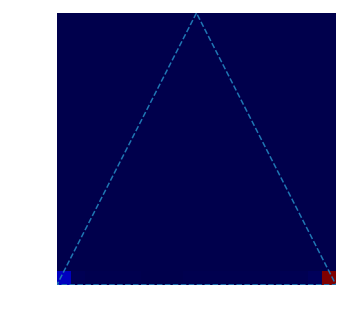
\includegraphics[width=\textwidth]{triangle_0_2kld.png}
\subcaption{}
\end{minipage}
 \begin{minipage}{.3\textwidth}
    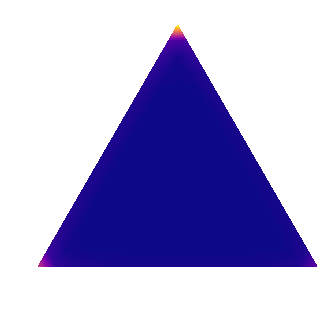
\includegraphics[width=\textwidth]{triangle_0_2elbo.png}
\subcaption{}
\end{minipage}
 \begin{minipage}{.3\textwidth}
    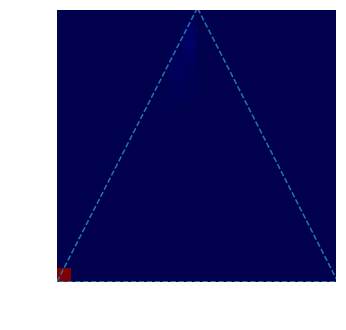
\includegraphics[width=\textwidth]{triangle_0_2overfit.png}
\subcaption{}
\end{minipage}

 \begin{minipage}[]{.3\textwidth}
    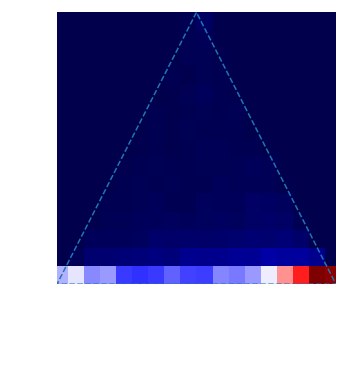
\includegraphics[width=\textwidth]{triangle_1kld.png}
\subcaption{}
\end{minipage}
 \begin{minipage}{.3\textwidth}
    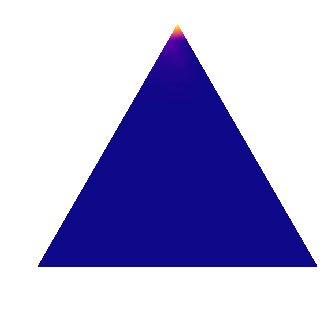
\includegraphics[width=\textwidth]{triangle_1elbo.png}
\subcaption{}
\end{minipage}
 \begin{minipage}{.3\textwidth}
    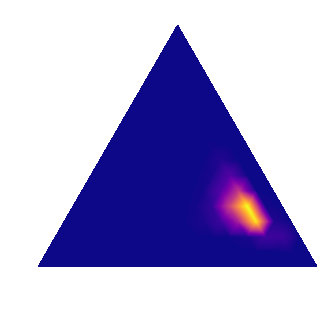
\includegraphics[width=\textwidth]{triangle_1overfit.png}
\subcaption{}
\end{minipage}


 \begin{minipage}[]{.3\textwidth}
    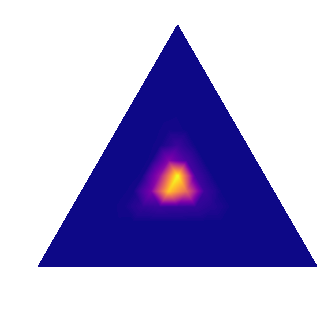
\includegraphics[width=\textwidth]{triangle_10kld.png}
\subcaption{}
\end{minipage}
 \begin{minipage}{.3\textwidth}
    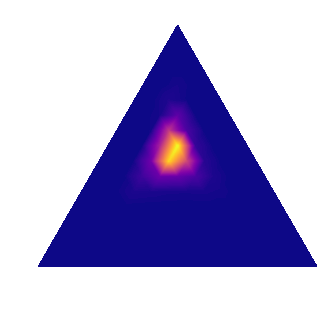
\includegraphics[width=\textwidth]{triangle_10elbo.png}
\subcaption{}
\end{minipage}
 \begin{minipage}{.3\textwidth}
    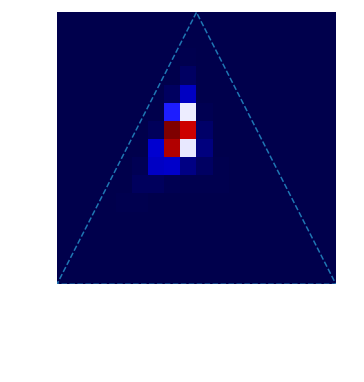
\includegraphics[width=\textwidth]{triangle_10overfit.png}
\subcaption{}
\end{minipage}
\caption{Гистограмма итогового вариационного распределения $\qG$ структур при различных значениях метапараметров. Левый нижний угол соответствует модели $\model_0$, верхний угол соответствет модели $\model_1$, правый нижний угол соответствует модели $\model_2$.
Первый столбец:  $\lamLL = 0.01, \lamCQ = 1, \lamCL = 100, \lamS = \mathbf{0},$  второй столбец: $\lamLL = \lamCL = \lamCQ = 1, \lamS = \mathbf{0},$ 
третий столбец: $\lamLL = 100.0, \lamCQ = 1, \lamCL = 0.01, \lamS = \mathbf{0}.$ 
Первая строка: $\lamT = 0.2$, вторая строка: $\lamT = 1.0$, третья строка: $\lamT = 10.0$.}
\label{fig:fig_triangle_hist}
\end{figure}


\begin{figure}
 \begin{minipage}[]{.3\textwidth}
    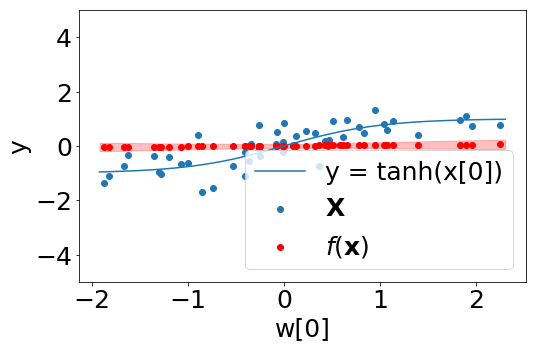
\includegraphics[width=\textwidth]{plot_0_2kld.png}
\subcaption{}
\end{minipage}
 \begin{minipage}{.3\textwidth}
    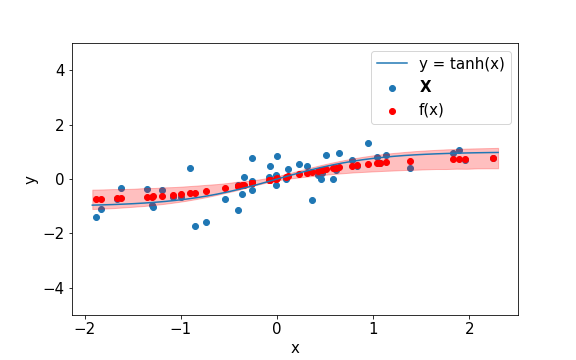
\includegraphics[width=\textwidth]{plot_0_2elbo.png}
\subcaption{}
\end{minipage}
 \begin{minipage}{.3\textwidth}
    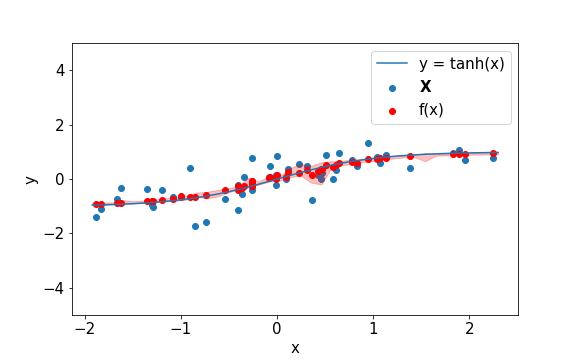
\includegraphics[width=\textwidth]{plot_0_2overfit.png}
\subcaption{}
\end{minipage}

 \begin{minipage}[]{.3\textwidth}
    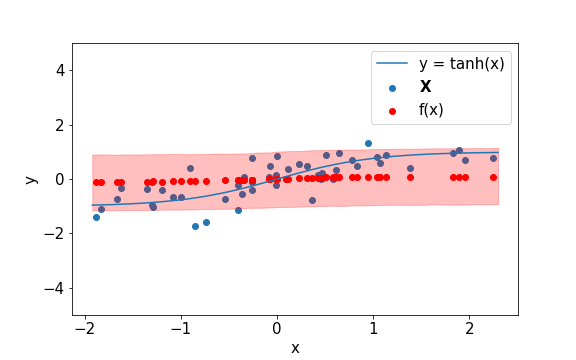
\includegraphics[width=\textwidth]{plot_1kld.png}
\subcaption{}
\end{minipage}
 \begin{minipage}{.3\textwidth}
    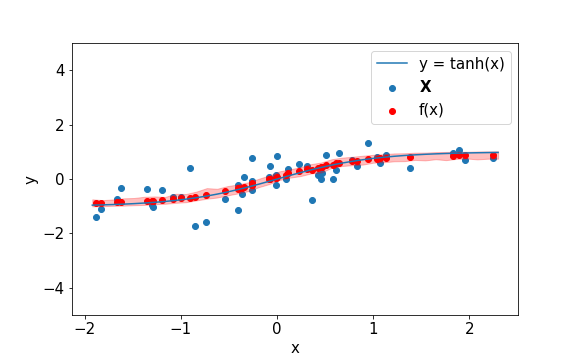
\includegraphics[width=\textwidth]{plot_1elbo.png}
\subcaption{}
\end{minipage}
 \begin{minipage}{.3\textwidth}
    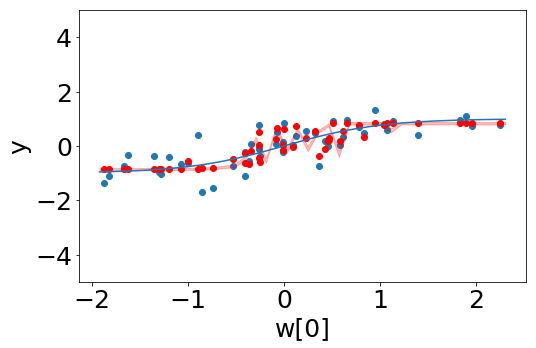
\includegraphics[width=\textwidth]{plot_1overfit.png}
\subcaption{}
\end{minipage}


 \begin{minipage}[]{.3\textwidth}
    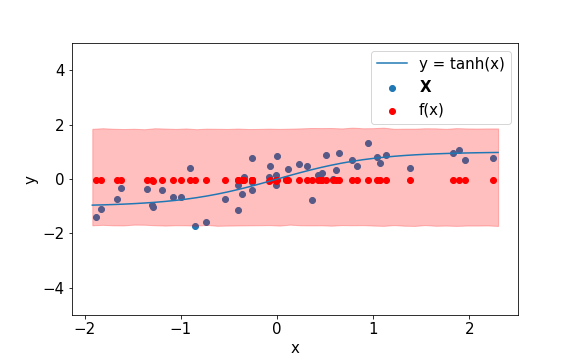
\includegraphics[width=\textwidth]{plot_10kld.png}
\subcaption{}
\end{minipage}
 \begin{minipage}{.3\textwidth}
    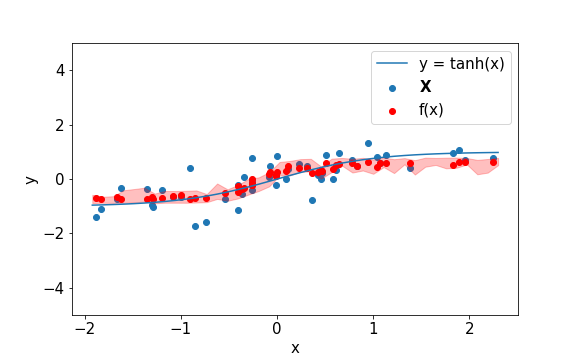
\includegraphics[width=\textwidth]{plot_10elbo.png}
\subcaption{}
\end{minipage}
 \begin{minipage}{.3\textwidth}
    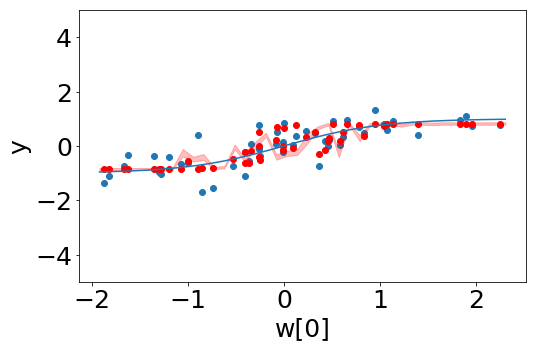
\includegraphics[width=\textwidth]{plot_10overfit.png}
\subcaption{}
\end{minipage}

\caption{График зависимости $\model$ от нулевой компоненты вектора $\x$ для итоговых моделей.
Первый столбец: $\lamLL = 0.01, \lamCQ = 1, \lamCL = 100, \lamS = \mathbf{0},$  второй столбец: $\lamLL = \lamCL = \lamCQ = 1, \lamS = \mathbf{0},$ 
третий столбец: $\lamLL = 100.0, \lamCQ = 1, \lamCL = 0.01, \lamS = \mathbf{0}.$ 
Первая строка: $\lamT = 0.2$, вторая строка: $\lamT = 1.0$, третья строка: $\lamT = 10.0$.}
\label{fig:fig_plot_synthetic_results}
\end{figure}




График относительной плотности~\eqref{eq:rho_graves} параметров моделей представлен на Рис.~\ref{fig:bar_rho}. Высокая относительная плотность параметров соответствует наиболее вероятным по вариационному распределению структурам.


\begin{figure}
 \begin{minipage}[]{.3\textwidth}
    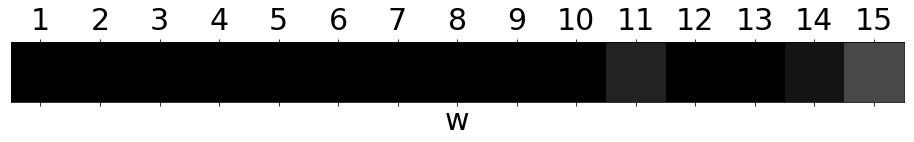
\includegraphics[width=\textwidth]{bar_0_2kld.png}
\subcaption{}
\end{minipage}
 \begin{minipage}{.3\textwidth}
    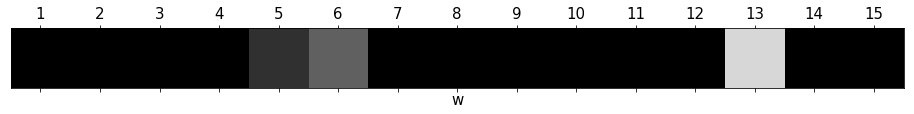
\includegraphics[width=\textwidth]{bar_0_2elbo.png}
\subcaption{}
\end{minipage}
 \begin{minipage}{.3\textwidth}
    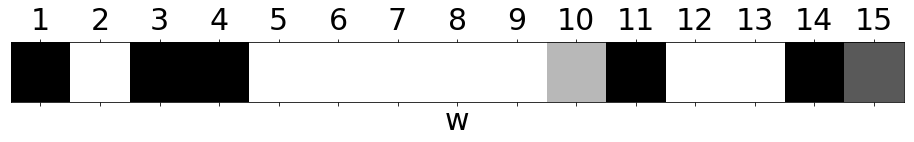
\includegraphics[width=\textwidth]{bar_0_2overfit.png}
\subcaption{}
\end{minipage}


\caption{Относительная плотность параметров итоговых моделей при $\lamT = 0.2$.
Первый столбец: $\lamLL = 0.01, \lamCQ = 1, \lamCL = 100, \lamS = \mathbf{0},$  второй столбец: $\lamLL = \lamCL = \lamCQ = 1, \lamS = \mathbf{0},$ 
третий столбец: $\lamLL = 100.0, \lamCQ = 1, \lamCL = 0.01, \lamS = \mathbf{0}.$ Первый параметр соответствует модели $\model_0$, второй и третий параметр соответствует модели $\model_1$, параметры 4-15 cоответствуют модели $\model_2$.}
\label{fig:bar_rho}
\end{figure}


Для анализа возможности перехода между структурами был проведен эксперимент с параметрами 
$\lamLL = 0.01, \lamCQ = 1, \lamCL = 100, \lamS = [-1, -1], \lamT = 1.0.$
В качестве структур $\mathfrak{P}$ выступали следующие структуры:
\[
    p_1  =  \mathcal{GS}(0.1, [0.99, 0.05, 0.05]), \quad p_2  =  \mathcal{GS}(0.1, [0.05, 0.05, 0.99]).
\]
Данные структуры соответствуют распределениям структур, сконцентрированным близко к моделям $\model_0, \model_2$.
Гистограмма итоговых распределений для данной задачи оптимизации представлена на Рис.~\ref{fig:structure_comb_example}.
График показывает, что в отличие от оптимизации с $\lamS=\mathbf{0}$, которая представлена на Рис.~\ref{fig:fig_triangle_hist}~д), при использовании данного слагаемого вариационное распределение $\qG$ сконцентрировано у модели $\model_1$.
Заметим, что данная регуляризация  влияет напрямую только на априорное распределение структур $\priorG$, а не на вариационное распределение $\qG$, поэтому итоговое распределение $\qG$ изменяется значительно только при близких значениях суммы остальных слагаемых обобщающей задачи оптимизации.




\begin{figure}
\centering
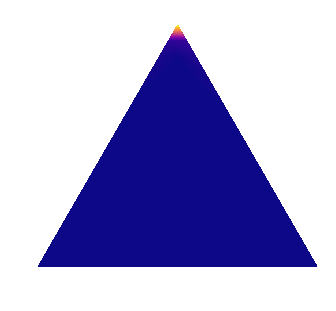
\includegraphics[width=0.2\textwidth]{triangle_structure_comb.png}
\caption{Оптимизация с метапраметром $\lamS=1.$}
\label{fig:structure_comb_example}
\end{figure}
